\cchapter{مقدمه}
\par
امروزه از روش‌های متعددی برای رأی‌گیری استفاده می‌شود. رأی‌گیری سنتی به کمک صندوق‌های رأی‌ و برگه‌ رأی‌های کاغذی انجام می‌شود. با توجه به سختی استفاده از این روش در انتخابات‌های بزرگ، فعالیت‌های زیادی در راستای رأی‌گیری الکترونیک انجام شده است. اولین سامانه‌ی رأی‌گیری الکترونیک در سال ۱۹۶۰ طراحی شده است و اولین استفاده‌ بزرگ از آن‌ها در چند ایالت آمریکا در سال ۱۹۶۴ برای انتخابات ریاست جمهوری بود. 

\par
امنیت در رأی‌گیری همواره یک مسئله‌ی پیچیده بوده است که در روش‌های سنتی به کمک بررسی‌های انسانی و اعتماد به برگزارکننده تامین می‌شده ولی به کمک رمزنگاری در رأی‌گیری الکترونیک می‌توانیم نیاز به شخص معتمد در رأی‌گیری را کمرنگ کنیم. هدف نهایی ما در این تحقیق ارائه‌ی یک روش رأی‌گیری امن بدون نیاز به اعتماد به شخص ثالث است. 
\section{نیازمندی‌های رأی‌گیری ایده‌آل}

یک فرایند‌ رأی‌گیری ایده‌آل باید بتواند شروط زیر را بدون نیاز به اعتماد به شخص ثالث ارضا کند:
\begin{itemize}
	\item 
	هر فرد واجد شرایط دقیقا یک بار بتواند رأی دهد.
	\item 
	هیچ کسی نتواند به جای فرد دیگری رأی دهد.
	\item 
  	هیچ فردی مجبور به رأی دادن نشود.
  	\item 
  	هیچ فردی مجبور به رأی دادن به کاندیدای خاصی نشود.
  	\item 
  	از شمارش هر رأی اطمینان حاصل شود.
  	\item 
    نتیجه‌ی رأیء ناشناس  باقی بماند. 
  	\item 
  	بسته به نیاز بتوان نتایج لحظه‌ای انتخابات را (بدون آسیب به شرط‌های قبلی) دید.
\end{itemize}

\section{روش‌های رأی‌گیری سنتی}
\par
در رأی‌گیری سنتی فرد برای رأی‌دادن به یکی از حوزه‌های رأی‌گیری مراجعه کرده و با ارائه‌ی مدارک شناسایی خود یک برگه‌ی رأی دریافت می‌کند. برگه رأی دارای دو بخش است: قسمتی که برای ردیابی با اطلاعات شخصی فرد پر می‌شود و یک قسمت بی‌نام که فرد کاندیدای مورد نظر خود را در آن ثبت کرده و در یک صندوق می‌اندازد. 
\\
با بررسی مدارک شناسایی، شرط دوم فرایند رأی‌گیری ایده‌آل تایید شده و با ثبت شدن اطلاعات فرد به عنوان یک رأی‌دهنده از رأی دادن دوباره‌ی او جلوگیری می‌شود. امنیت شخصی افراد در حوزه توسط برگزارکننده‌ی انتخابات و پلیس تامین می‌شود و در صورتی که فردی به تحت فشار مجبور به مراجعه به حوزه‌ی رأی‌گیری شده باشد می‌تواند با گزینه‌ی «رأی‌ سفید» از رأی دادن خودداری کند.
\\
با وجود یک صندوق برای چندین رأی و نبودن هیچ نشانه‌ی شناسایی در رأیء، هیچ راهی برای فهمیدن رأی یک فرد خاص - حتی اگر برگه‌های رأی به دست رقیب بیفتد - وجود ندارد. 
\\
احزار هویت و شمارش رأی‌ها به عهده‌ی برگزارکننده‌ی انتخابات است و تنها از طریق یک شخص ثالث برای باز‌شماری رأیء می‌توان از اجرای درست آن‌ها اطمینان حاصل کرد.
\\
با توجه به هزینه‌ی زیاد شمارش در انتخابات‌های بزرگ راهی برای اعلام لحظه‌ا‌ی نتایج با هزینه‌ی معقول وجود ندارد.
\\
همانطور که می‌بینیم در روش‌های فعلی انتخابات بسیاری از شرایط مورد نیاز یک انتخابات خوب  با هزینه‌ی نسبتا زیاد فراهم می‌شود. از دیگر مشکلات انتخابات به این روش می‌توان به نیازمندی به یک برگزارکننده‌ی مورد اعتماد اشاره کرد. باید به برگزارکننده اعتماد شود تا: 
\begin{enumerate}
	\item 
	امنیت حوزه‌ی انتخابات را تامین کند.
	\item 
	افراد را به درستی احراز هویت کند.
	\item 
	همه‌ی رأی‌ها را بشمرد.
	\item 
	تغییری در رأی‌ها ندهد.
	
\end{enumerate}
 

\section{مشکلات و چالش‌های رأی‌گیری الکترونیک}
\par
دو مسئله‌ی اساسی در یک رأی‌گیری امنیت و حریم خصوصی است. مخالفین رأی‌گیری الکترونیک از کم هزینه بودن تقلب و تغییر رأی‌های ثبت شده در انتخابات الکترونیک می‌گویند و رد کاغذی در یک انتخابات را یک فاکتور مهم برای امنیت آن می‌دانند. هزینه تغییر میلیون‌ها رأی در یک سامانه‌ی کامپیوتری بسیار پایین‌تر از تولید چند میلیون رأی کاغذی تقلبی برای تغییر نتیجه‌ی یک انتخابات است.
\\
بزرگترین مسئله در به‌کارگیری رأی‌گیری الکترونیک مسئله‌ی اعتماد به یک سامانه‌ی‌ کامپیوتری است. از نظر بسیاری از رأی‌دهندگان رأی دادن با کامپیوتر شخصی می‌تواند ریسک تغییر رأی تا رسیدن آن به سرور‌های رأی‌گیری ایجاد کند. از طرف دیگر عدم امکان بررسی و تایید انسانی عملیات کامپیوتر، حس امنیت کمتری القا می‌کند.
\par
مسئله‌ی دیگر پرهزینه بودن ساخت زیرساخت‌های رأی‌گیری الکترونیک و خطر پیدایش مشکلات امنیتی در هر سامانه‌ی کامپیوتری - چه از نظر نرم‌افزار و چه سخت‌افزار - است. این مشکل باعث شده تعدادی از کشور‌ها از جمله هلند، ایرلند و آلمان فرایند ایجاد زیرساخت لازم را شروع کرده و در ادامه این فرایند را ملقی کنند. دلیل اصلی اعلام شده برای این مسائل‌ قابل اتکا نبودن سامانه‌های رأی‌گیری الکترونیک اعلام شده است. 
\\
برای مثال یک تحقیق معروف از دانشگاه‌ \lr{NYU} در سال ۲۰۱۵ 
\LTRfootnote{https://www.brennancenter.org/publication/americas-voting-machines-risk}
توضیح داد که ماشین‌های رأی‌گیری الکترونیک که در ۴۳ ایالت آمریکا استفاده می‌شوند در سال ۲۰۱۶ به دهمین سال استفاده شدن می‌رسند و به دلیل نداشتن بودجه‌ی کافی برای تعمیرات و بروزرسانی، در معرض خطر کرش
\LTRfootnote{crash}
 کردن هستند که می‌تواند باعث کندی فرایند و حتی گاها از دست رفتن را‌ی‌های مردم شود. علاوه بر این، قدیمی بودن دستگاه‌ها می‌تواند ریسک‌های امنیتی ایحاد کند. 

\par
یک مشکل دیگر در پیاده‌سازی‌های بسیاری از رأی‌گیری الکترونیک، نیاز به اینترنت و توانایی استفاده از کامپیوتر است. این مسئله می‌تواند دسترسی بسیاری از افرادی واجد شرایط را - به دلیل نقص جسمی و یا عدم توانایی کار با کامپیوتر - محدود کند. در سامانه‌های فعلی که مبتنی بر حوزه‌های رأی‌گیری هستند می‌توانند با کمک انسانی در خود حوزه تا حدی این مشکلات را رفع کنند. 
\par
مشکلات مطرح‌ شده موانع بزرگی برای فراگیری سامانه‌های رأی‌گیری کاملا الکترونیکی برای انتخابات‌های مهم و بزرگ هستند که یک سامانه رأی‌گیری مناسب باید آن‌ها را تا جای ممکن رفع کند. 

\section{انگیزه و هدف}
هدف این تحقیق، طراحی یک سامانه‌ی رأی‌گیری الکترونیک است که شرایط رأی‌گیری ایده‌آل را تا جای ممکن بدون نیاز به اعتماد به شخص ثالث ارضا کند. با فراگیری تکنولوژی زنجیره‌ی قالبی برای ایجاد سامانه‌های توزیع شده بدون نیاز به اعتماد (برای مثال بیت‌کوین به عنوان یک‌ ارز دیجیتال بدون نیاز به اعتماد)، پلتفرم‌هایی برای رأی‌گیری الکترونیک ایجاد شدند که امنیت شمارش رأیء را با عمومی ساختن فرایند رأی‌گیری تامین می‌کردند. 
\\
با وجودی که راه‌حل ارائه شده‌ی این روش‌ها مسئله‌ی اطمینان از شمارش رأی‌ها را حل می‌کرد، مسئله‌ی حریم شخصی در این روش‌ها حل نشده است و انتخابات‌های برگزار شده با این سامانه‌ها امنیت کمتری در قبال ناشناس ماندن رأی‌ها ارائه می‌کنند. 
\\
برای مثال حالتی را فرض کنید که یک رأی‌دهنده تهدید می‌شود که باید به یک کاندیدای خاص رأی بدهد، در روش‌های سنتی رأی‌گیری به دلیل بی‌نام بودن برگه‌های رأی بعد از اتمام فرایند رأی‌گیری راهی برای اطمینان حاصل کردن از نتیجه‌ی رأی فرد نیست. از طرفی به دلیل امنیت حوزه‌های رأی‌گیری راهی برای اطمینان از نتیجه‌ی رأی یک نفر در حین فرایند رأی‌گیری هم نیست. پس راهی برای مجبور کردن یک نفر که به یک کاندیدای خاص رأی بدهد وجود ندارد. اما در سامانه‌های مبتنی بر زنجیره‌ی قالبی هر رأی داده شده با امضای الکترونیکی فرد امضا شده است و این موضوع می‌تواند با عمومی شدن زنجیره‌ی قالبی بعد از رأی‌گیری باعث لو رفتن نتیجه‌ی رأی آن فرد شود.
\\
این مشکلات مانع بزرگی برای استفاده‌ی فراگیر این روش‌ها خواهد بود. هدف ما در این تحقیق این است که سامانه‌ای ارائه کنیم که امنیت شمرده شدن رأیء را، مانند این سامانه‌ها ارائه کند و در عین حالت حریم خصوصی رأی‌دهنده را به طور کامل حفظ کند. 
\par
نتیجه‌ی این تحقیق یک روش‌ رأی‌گیری الکترونیک است که قیاس با روش‌های سنتی انتخابات هزینه‌ها را کاهش خواهد داد. در عین حال کمترین تغییر برای رأی‌دهندگان خواهد داشت که باعث افزایش دسترس‌پذیری این سامانه خواهد شد. همچنین تمامی رأیء رأی‌دهندگان در قبال یک مهاجم خارجی و حتی خود برگزار کننده‌ی انتخابات ناشناس خواهند ماند. 
\\
با این وجود این سامانه یک رد الکترونیک غیرقابل انکار از تمام ارا، در قالب یک زنجیره‌ی قالبی، ارائه ‌خواهد کرد که با وجود حفظ حریم خصوصی به هر ناظر ثالثی اثبات کند که رأیء درست شمرده شده است. همچنین تمامی این قابلیت‌ها بدون نیاز اعتماد به برگزارکننده‌ی انتخابات خواهد بود و هرگونه تخطی از پروتکل ارائه شده توسط حوزه‌های رأی‌گیری از طریق اطلاعات ثبت شده در زنجیره‌ی قالبی قابل ردیابی خواهد بود.








\cchapter{تعریف مفاهیم}
در این بخش به معرفی بعضی مفاهیم پایه‌ی به کار برده شده در این تحقیق می‌پردازیم. در ابتدا با مفاهیم زنجیره‌ی قالبی، انواع و کاربرد‌های آن آشنا می‌شویم و در ادامه به بررسی اثبات‌های بی‌دانش می‌پردازیم. این دو تکنولوژی ابزارهای تئوری لازم برای ساخت سامانه رأی‌گیری امن خواهند بود.
\section{زنجیره‌ی قالبی}
زنجیره‌ی قالبی ساختمان‌داده‌ایست که به مانند لینک‌‌لیست
\LTRfootnote{Linked list}
از بلوک‌‌های متوالی تشکیل شده ولی در زنجیره‌ی قالبی هر بلوک هش
\LTRfootnote{Hash}
عنصر قبلی خود را نیز نگه ‌می‌دارد. هدف از این کار ساخت یک ساختارداده‌ی صرفا افزایشی 
\LTRfootnote{Append only}
است که در آن‌ بلوک‌های قبلی تغییرناپذیرند. تغییر هر بلوک باعث تغییر بلوک بعدی خواهد شد و این موضوع تشخیص تغییر در بلوک‌های پیشین را بسیار ساده می‌کند.
\subsection{پیاده‌سازی زنجیره‌ی قالبی}


برای پیاده‌سازی یک زنجیره‌ی قالبی معمولا از درخت مرکل
 \LTRfootnote{Merkle tree}
 استفاده‌ می‌شود؛ درخت مرکل یا درخت هش، نوعی درخت دودویی 
 \LTRfootnote{Binary tree}
 است که در آن هر راس هش فرزندان خود را نگه ‌داشته و برگ‌ها هش داده‌ی ذخیره‌شده در خودشان را نگه می‌دارند. این روش نگهداری اطلاعات باعث می‌شود که درچه‌ی زمانی بررسی وجود یک بلوک داده در زنجیره‌ی قالبی از 
 \lr{N}
 به 
$ \log N$
 کاهش یابد. با توجه به این نوع ساختار درخت مرکل، هر تغییری در درخت باعت تغییر هش در ریشه‌ی آن خواهد شد و به دلیل تصادفی بودن خروجی یک هش خوب، هش ریشه‌ی درخت مرکل هیچ ویژگی قابل پیشبینی ندارد.
 
 \begin{figure}[th!]
 	\centering
 	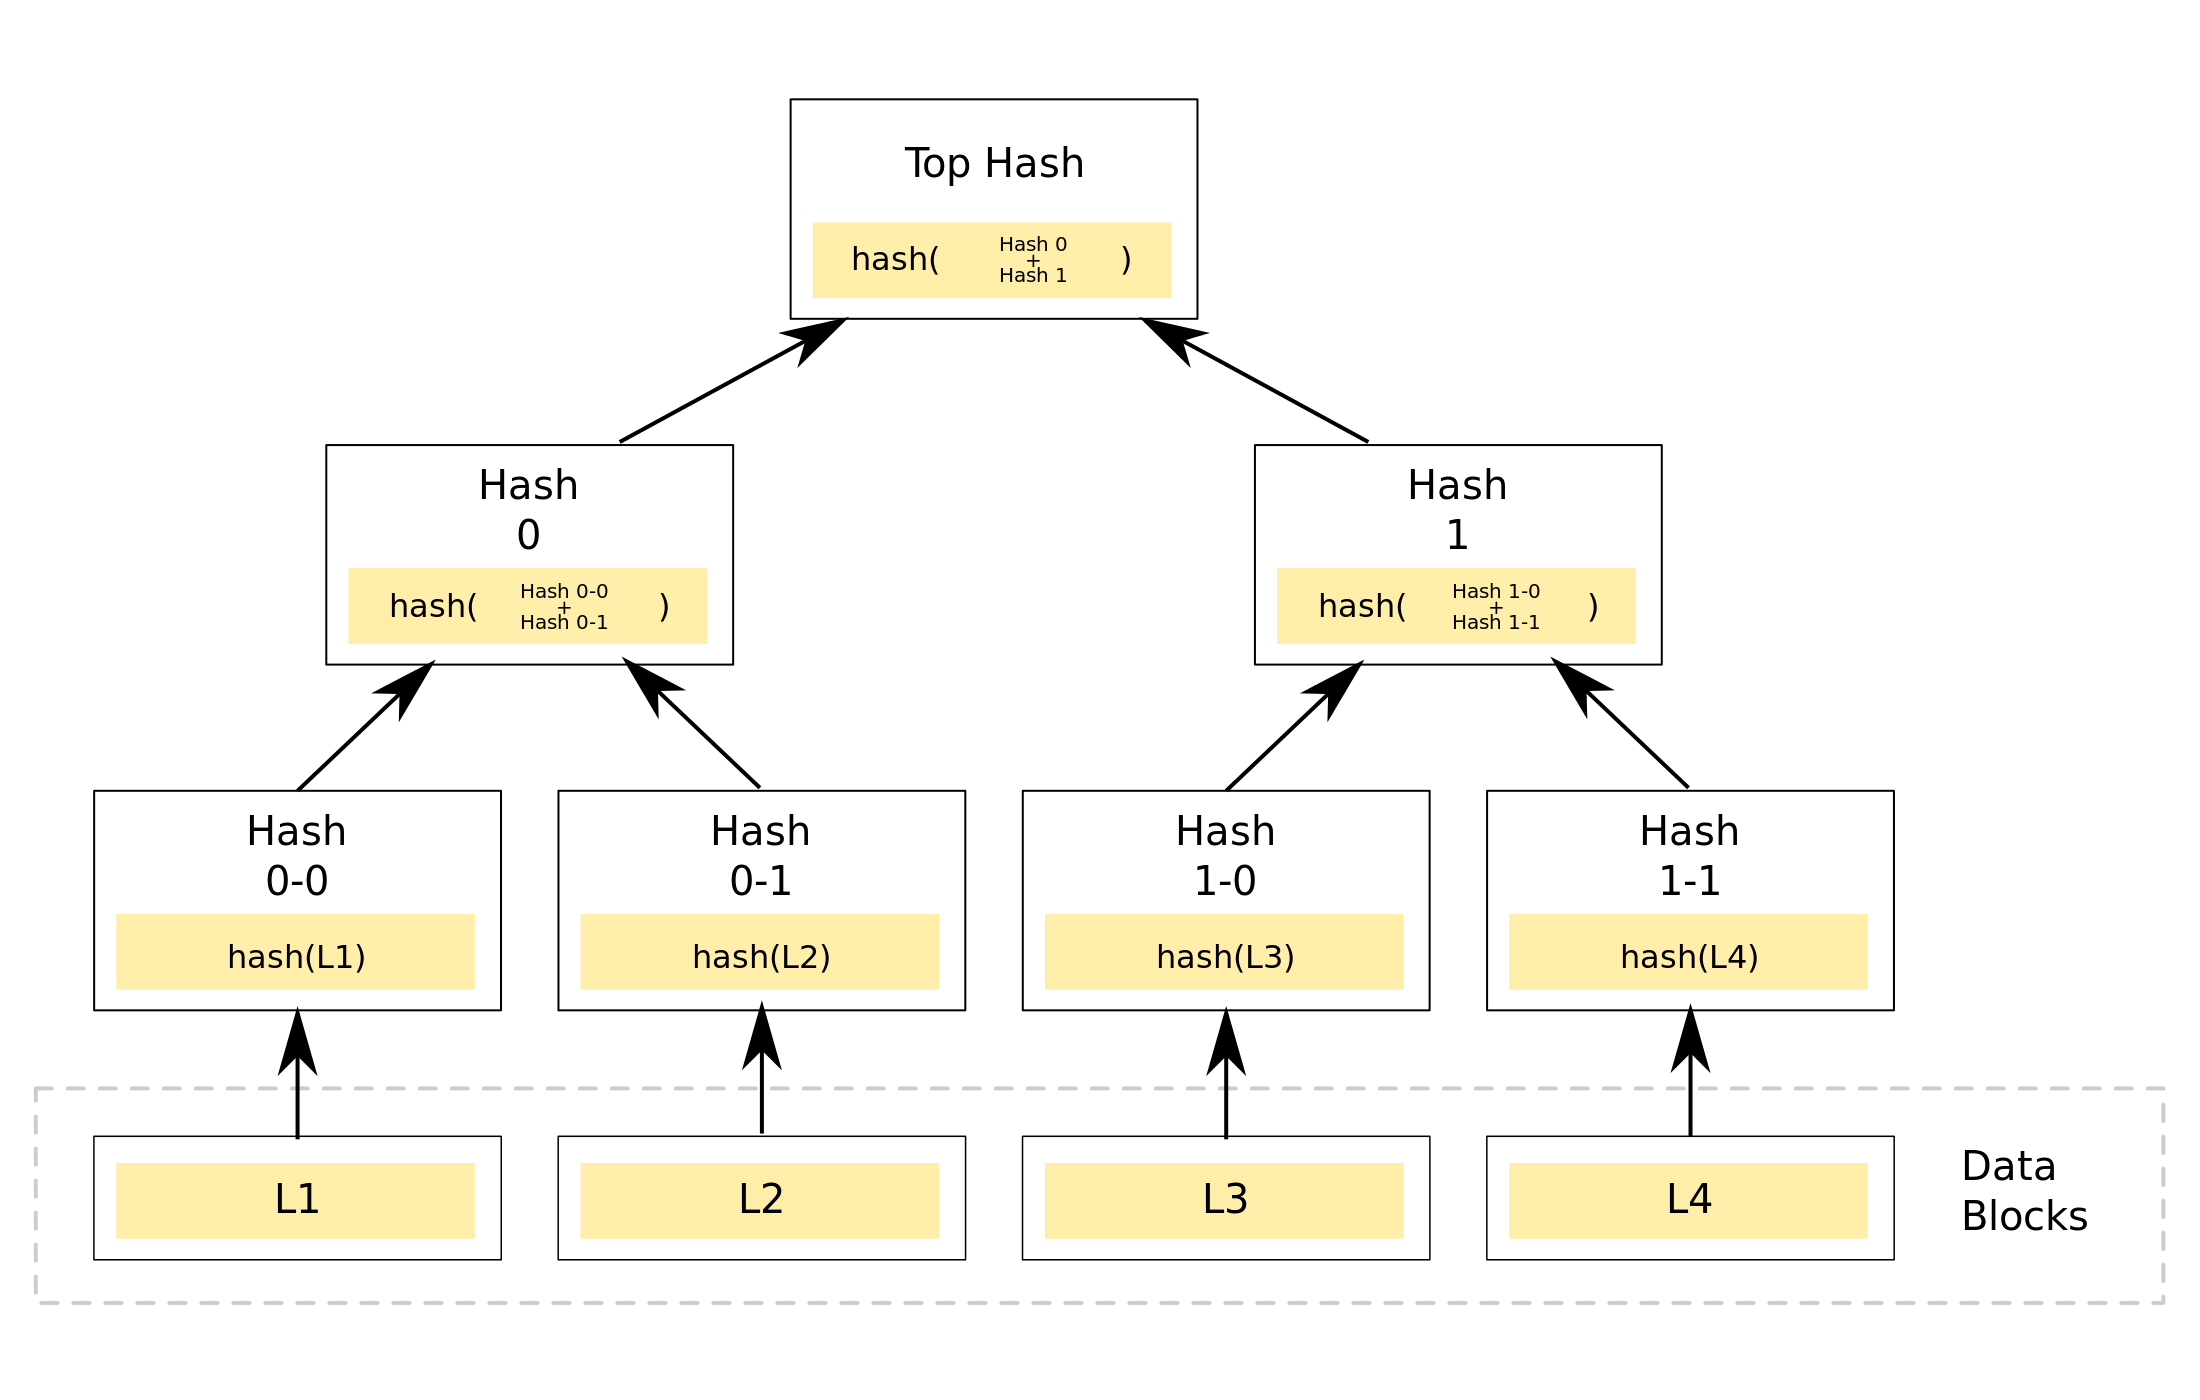
\includegraphics[width=.7\linewidth]{Hash_Tree.png}
 	\caption {یک درخت مرکل}
 	\label{fig:merkle}
 \end{figure}
 
 \subsection{انواع زنجیره‌ی قالبی}
 در این تحقیق زنجیره‌های قالبی‌ را از دو نظر دسته‌‌بندی می‌کنیم. زنجیره‌های قالبی‌ می‌توانند عمومی یا خصوصی باشند، در زنجیره‌های قالبی‌ عمومی اضافه‌کردن بلوک به زنجیره‌ی قالبی نیاز به دسترسی خاصی ندارد و هر کسی می‌تواند در آن‌ها بنویسد ولی در زنجیره‌های قالبی خصوصی اضافه کردن بلوک تنها توسط افراد خاص ممکن است. 
 \\
 روش دیگر تقسیم‌بندی ما باز یا بسته بودن زنجیره‌ی قالبی است که در رایطه با دسترسی خواندن اطلاعات در این زنجیره می‌باشد. در زنجیره‌های قالبی‌ بسته خواندن اطلاعات توسط عموم آزاد نیست. در حالی که دو نوع باز آن تمام اطلاعات زنجیره برای خواندن در دسترس عموم است.
\par
با توجه به کاربرد زنجیره‌ی قالبی مورد نظر هر زنجیره‌ می‌تواند در هر یک از این دسته‌بندی‌ها قرار بگیرد. جدول  \ref{tab:tch} یک کاربرد ممکن برای هر کدام از این دسته‌بندی‌ها را نشان می‌دهد.

\begin{table}[h]
	\begin{center}
		%		\def\arraystretch{2}
		\caption{انواع زنجیره‌ی قالبی}
		\begin{tabular}{|c|c|c|}
			\hline
			& باز & بسته \\
			\hline
			عمومی & ارز‌های دیجیتال & بعضی رأی‌گیری‌ها \\
			\hline
			خصوصی & سامانه‌ی مدیریت اطلاعات مالیات & اطلاعات خصوصی یک شرکت \\
			\hline

		\end{tabular}
		\label{tab:tch}
	\end{center}
\end{table}


 
 
\section{اثبات‌های بی‌دانش}
اثبات‌ بی‌دانش 
\LTRfootnote{Zero knowledge proofs}
روشی است که در آن «اثبات‌کننده» می‌تواند یه «بررسی‌کننده» نشان دهد که او یک راز - مثلا خروجی یک عملیات کامپیوتری - را می‌داند، بدون این که به او هیچ اطلاعات اضافه‌ای، مانند خروجی عملیات، بدهد. به عبارت دیگر اثبات‌های بی‌دانش، صرفا داشتن اطلاعات را اثبات می‌کنند و خود اطلاعات را محفوظ نگه‌ می‌دارند.
\\
یک اثبات بی‌دانش باید ۳ شرط زیر را داشته باشد:
\begin{itemize}
	\item
	کامل‌بودن: اگر گزاره‌ی مورد اثبات صحیح باشد، بررسی‌کننده‌ای که پروتکل را رعایت کند، باید از درستی گزاره مطمئن شود.
	\item 
	درستی: اگر گزاره مورد اثبات غلط باشد، هیچ اثبات‌کننده‌ای نتواند اثباتی در رابطه با درست بودن گزاره ارائه کند.
	\item 
	بی‌دانش: اگر اثبات درست باشد، بررسی‌کننده هیچ اطلاعاتی فراتر از درست بودن گزاره دریافت نکند.
\end{itemize}
اثبات‌های بی‌دانش، اثبات‌های احتمالاتی هستند و در واقع احتمال کمی وجود دارد که بتوان یک اثبات نادرست ارائه کرد. به بیان دیگر شرط درستی این است که احتمال تولید یک اثبات نادرست بسیار کم باشد. 
\subsection{مثال شهودی}
سناریویی را در نظر می‌گیریم که یک توپ سبز و یک توپ قرمز روی یک میز قرار دارد و آلیس می‌خواهد به باب که کوررنگ سبز و قرمز است ثابت کند که این دو توپ با هم تفاوت دارند؛ برای اثبات آلیس چشمش را می‌بندد و باب یا دو توپ را جابجا می‌کند و یا جابجا نمی‌کند. در ادامه آلیس می‌گوید که آیا جای توپ‌ها با هم عوض شده‌اند یا نه. با یک پاسخ درست باب می‌فهمد که آلیس با احتمال ۵۰٪ درست می‌گوید. این فرایند را برای بار دوم نیز تکرار می‌کنند و در صورتی درست بودن جواب آلیس، باب می‌داند که با احتمال ۷۵٪ او تفاوتی بین دو توپ می‌بیند. این فرایند آنقدر تکرار می‌شود تا باب با احتمال دلخواه خود از ادعای آلیس اطمینان حاصل کند.
\par
نکته‌ی مهم در مثال بالا این است که حتی اگر باب این فرایند را ضبط کرده باشد، نمی‌تواند به کس دیگری ثابت کند که آلیس تفاوت این دو توپ را می‌داند چون که راهی برای اثبات این که سوال و جواب از قبل هماهنگ نشده بوده است ندارد. 
\\
این یکی از نیازمندی‌های بی‌دانش بودن اثبات است. اگر در طول فرایند باب برای تصمیم‌گیری در تعویض کردن یا نکردن توپ‌ها از شیر یا خط کردن یک سکه استفاده می‌کرد، دیگر این اثبات بی‌دانش نبود، چرا که باب می‌توانست با ضبط کردن این فرایند به یک شخص ثالث اثبات کند که آلیس تفاوت این دو توپ را می‌داند. 
\\
برای داشتن شرط بالا یک اثبات بی‌دانش همواره به تعامل از سمت بررسی‌کننده نیاز دارد. اما با ریلکس کردن این شرط و استفاده از یک ورودی غیرقابل پیشبینی برای تولید سوال‌های یک اثبات بی‌دانش - مثلا هش ریشه‌ی یک درخت مرکل - می‌توان اثبات‌های بی‌دانش بدون نیاز به تعامل بررسی‌کننده ساخت. 


\subsection{اثبات‌های بی‌دانش بدون تعامل} 
منظور از اثبات بدون تعامل، اثباتی‌ است که در آن نیازی به فرستادن پیام از سمت بررسی‌کننده به اثبات‌کننده نباشد. با این روش‌ها اثبات‌کننده می‌تواند اثبات را مستقل از بررسی‌کننده بسازد و ارسال کند. در ادامه‌ی این تحقیق اثبات‌های بی‌دانش و بی‌تعامل را 
\textbf{شاهد}
می‌نامیم. همچنین دو روش تولید یک شاهد بی‌دانش را بررسی می‌کنیم. این روش‌ها می‌توانند برای خروجی هر محاسبات کامپیوتری شاهد ایجاد کنند. 

\subsubsection{اثبات بی‌دانش \lr{ZK-SNARK}}
یکی از پرکاربردترین روش‌های ایجاد شاهد، 
\lr{ZK-SٔNARK}
\LTRfootnote{Zero-Knowledge Succint Non-Interactive Argument of Knowlege}
\cite{zksnark}
است. شاهد‌های این روش علاوه بر بی‌دانش بودن ویژگی‌های زیر را دارند:
\begin{itemize}
	\item 
	مختصر
	\LTRfootnote{Succinct}
	: تولید و بررسی شاهد از انجام محاسباتی که اثبات می‌شود کوتاه‌تر (معمولا از مرتبه‌ی زمانی $ (\log N) ^ 2$) است. 
	\item
	بی‌تعامل
	\LTRfootnote{Non-Interactive}
	: نیازی به پیامی از بررسی‌کننده برای تولید شاهد نیست. 
	\item
	ادعای دانش
	\LTRfootnote{Argument of Knowledge}
	: اثبات ارائه شده در این روش درست 
	\LTRfootnote{Sound}
	است و نمی‌توان بدون داشتن اطلاعات آن را در زمان محدود ساخت.
	
\end{itemize}
 
\begin{figure}[bh]
	\centering
	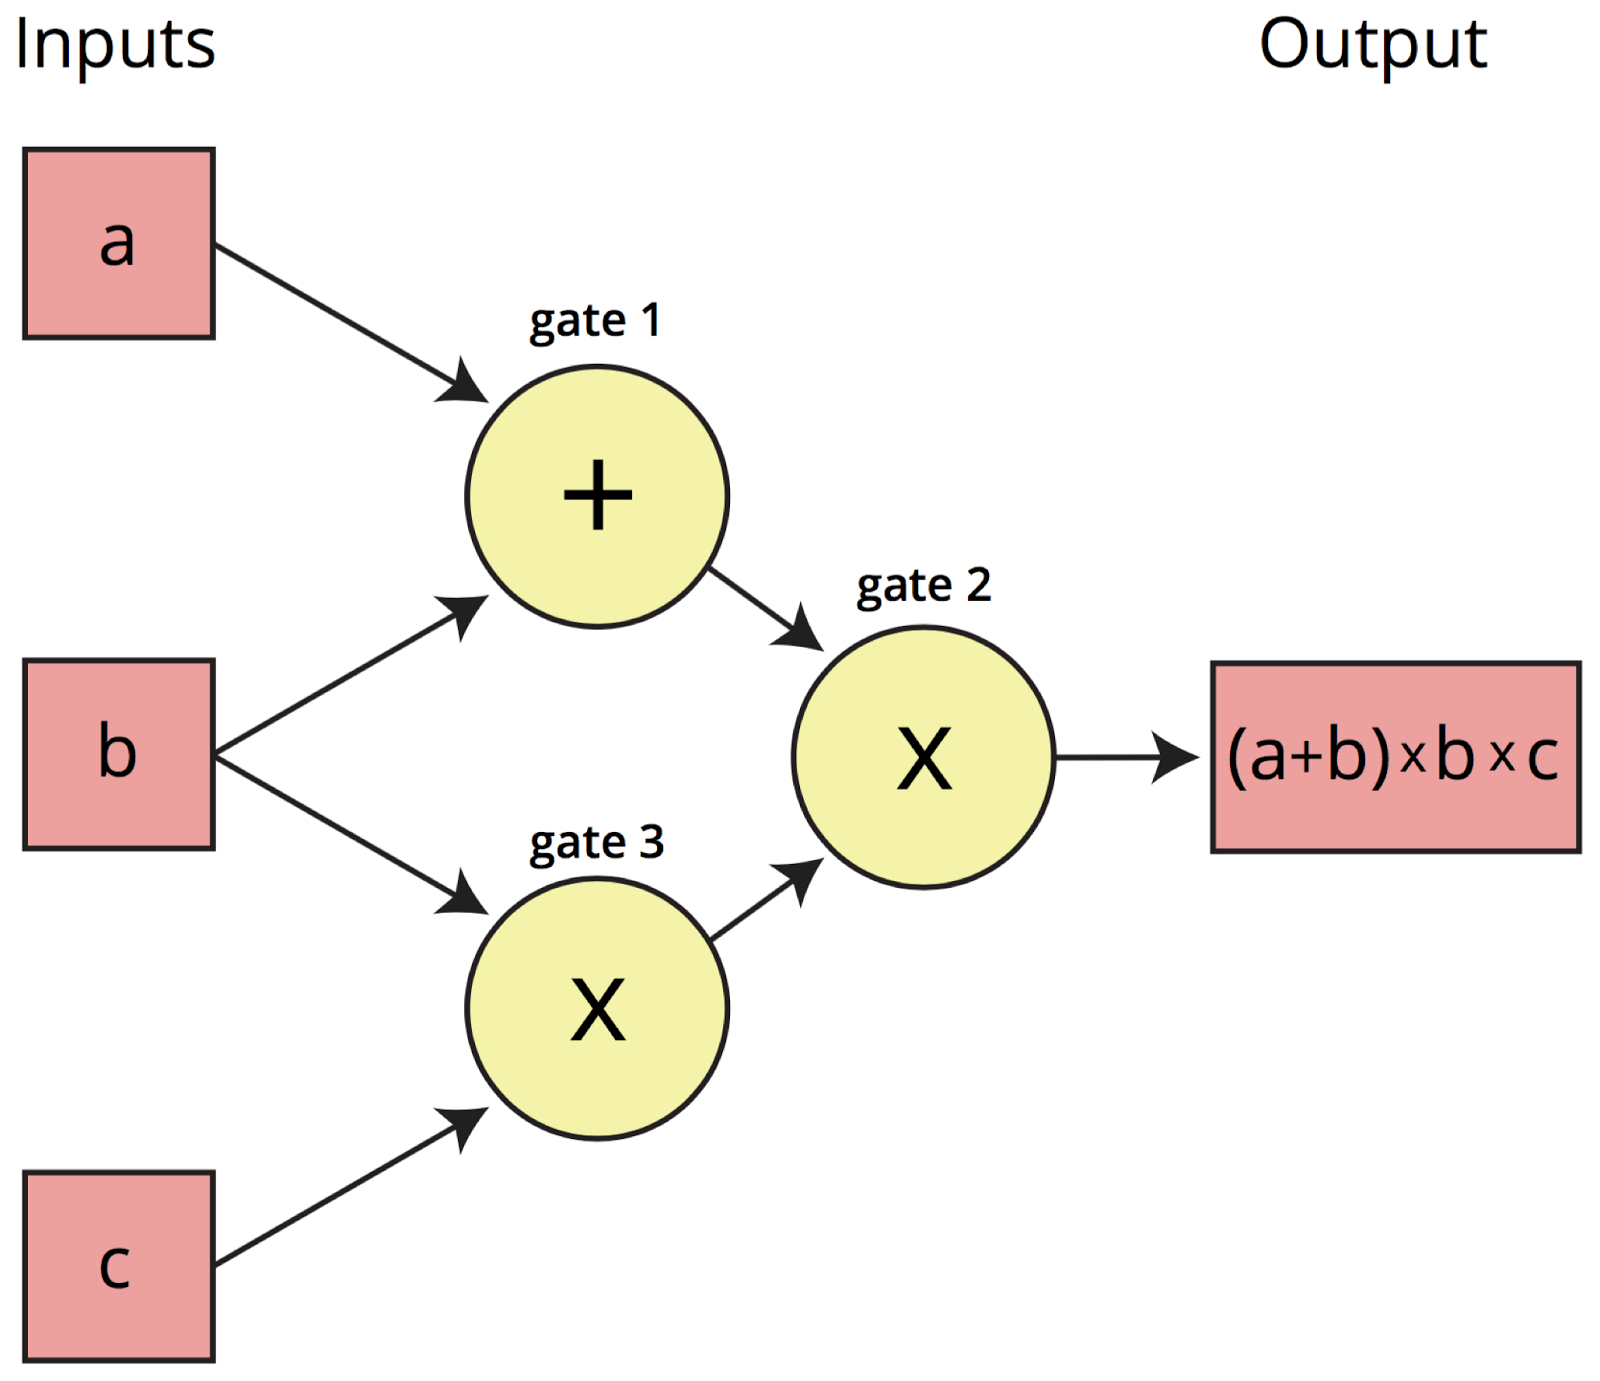
\includegraphics[width=.5\linewidth]{arithmetic-circuit.png}
	\caption {یک نمونه مدار محاسباتی}
	\label{fig:arithmetic}
\end{figure}

برای ساختن یک شاهد به این روش ابتدا محاسبات لازم را به یک مدار محاسباتی ریاضی تبدیل می‌کنیم به طوری که اثبات را به عنوان تعدادی شرط روی این مدار نشان دهیم، سپس به کمک یک
\lr{elliptic curve}
مقدار مدار را در چند نقطه‌ی تصادفی به عنوان اثبات ارائه می‌کنیم و با صادق بودن شرط‌ها در این نقاط شاهد را بررسی می‌کنیم. 
\\
برای انتخاب یکسان این نقاط تصادفی بین اثبات‌کننده و بررسی‌کننده نیاز به تعدادی نقطه‌ی توافق شده روی \lr{elliptic curve} داریم که باید قبل از تولید اثبات انتخاب شده باشند. در این فاز آماده‌سازی تعدادی عدد تصادفی برای انتخاب این نقاط تولید می‌شوند که بعد از آن باید بلافاصله پاک شوند. کسی که این اعداد (در واقع نقطه‌ی شروع روی منحنی) را داشته باشد می‌تواند شاهد‌های تقلبی ایجاد کند. برای تولید شاهد واقعی نیازی به دانستن این نقاط نیست. بنابراین بعد از فاز آماده‌سازی این اعداد باید پاک شوند. 
\subsubsection{اثبات بی‌دانش \lr{ZK-STARK}}
از روش‌های دیگر ایجاد شاهد بی‌دانش روش \lr{ZK-STARK}
\LTRfootnote{Zero-Knowledge Scalable Transparent ARguments of Knowledge}
\cite{zkstark}
است. مهم‌ترین وجه تمایز این روش در مقایسه با
\lr{ZK-SNARK}
 «شفافیت»
 \LTRfootnote{Transparency}
است. به این معنی که نیازی به فاز آماده‌سازی ندارد. عدم نیاز به آماده‌سازی و نداشتن زباله‌ی سمی (اطلاعاتی که باید پاک شوند تا امنیت سامانه تامین شود) این روش را برای کاربرد‌های حساس مناسب‌تر می‌کند اما در ازای این امنیت، حجم شاهد‌ها از چند صد بایت به چند صد هزار بایت تغییر می‌کند.
\par
ار مزیت‌های دیگر این روش استفاده نکردن از 
\lr{Elliptic curve}ها
است. نیاز‌های کم این روش باعث می‌شود که حتی با کامپیوتر‌های کوانتمی
\LTRfootnote{Quantum computers}
 راهی برای شکستن این اثبات‌ها وجود نداشته باشد.
\\
برای ساختن یک شاهد با این روش، برنامه‌ی مورد نظر را تبدیل یه یک چندجمله‌ای درجه بالا می‌کنند، سپس از مقادیر خروجی این چندجمله‌ای یک درخت مرکل ساخته می‌شود که خروجی‌های چند‌جمله‌ای را به ازای ورودی‌های مختلف نشان می‌دهد. سپس بررسی‌کننده چند شاخه از این درخت را به طور تصادفی انتخاب و بررسی می‌کند. برای غیرتعاملی کردن این اثبات می‌توان از هش ریشه‌ی درخت مرکل به عنوان ورودی یه تابع شبه‌تصادفی
\LTRfootnote{Pseudo random}
استفاده می‌شود که مشخص می‌کند خروجی کدام شاخه‌ها باید در شاهد ظاهر شود. 





\cchapter{کارهای پیشین}

از آن‌جایی که مهمترین خصوصیت‌های یک سامانه رأی‌گیری مناسب امنیت شمارش رأیء و حفظ حریم خصوصی رأی‌دهنده است، این دو موضوع پایه‌های طراحی یک سامانه رأی‌گیری امن خواهند بود. سامانه‌های رأی‌گیری الکترونیک قبل از تکنولوژی زنجیره‌ی قالبی از روش‌های متعددی برای تحقق این هدف استفاده می‌کردند اما تقریبا در تمامی این روش‌ها نیاز به اعتماد به مجری انتخابات وجود دارد. 
\par
طراحی زنجیره‌های قالبی همراه به کمک روش‌های توافق خلاقانه باعث ایجاد ارز‌های دیجیتال بدون نیاز به یک شخص (بانک) مورد اعتماد شد. در ادامه این ساختارداده‌ی اکیدا افزایشی برای حذف نیاز به اعتماد در کاربدهای دیگر نیز استفاده شده است. زنجیره‌ی قالبی در این تحقیق نیز به عنوانی ابزاری که با ایجاد شفافیت نیاز به اعتماد را کاهش می‌دهند استفاده می‌شود.
\par 
شفافیت در انتخابات خود باعث ایجاد مشکلاتی برای امنیت رأی‌دهندگان می‌شود. عدم حفظ حریم خصوصی رأی‌دهنده در یک انتخابات می‌تواند باعث شود رأی‌دهنده نتواند به کاندیدای دلخواهش رأی دهد یا تحت فشار مجبور به رأی‌دادن شود. برای رفع این مسئله از روش‌هایی مانند اثبات‌های بی‌دانش استفاده می‌شود. اثبات‌های بی‌دانش این امکان را ایجاد می‌کنند تا حتی با حفظ حریم خصوصی کاربر، درستی شمارش انتخابات اثبات گردد.
\par
در این بخش ابتدا روش‌های مختلف رأی‌گیری الکترونیک را بررسی می‌کنم و روش‌های استفاده شده برای حفظ امنیت و حریم خصوصی را تحلیل می‌کنیم. در ادامه تکنولوژی زنجیره‌ی قالبی را به عنوان ابزاری برای کاهش نیاز به اعتماد و ایجاد شفافیت بررسی می‌کنیم و در نهایت اثبات‌های بی‌دانش را به هدف ناشناس نگه‌ داشتن رأی‌گیری بررسی می‌کنیم.

\section{رأی‌گیری الکترونیک}
رأی‌گیری الکترونیک را به طور کلی ‌‌توانیم به دو دسته‌ی رأی‌گیری تماما الکترونیک و رأی‌گیری به کمک ابزار‌های الکترونیکی تقسیم کرد. روش‌های دسته‌ی دوم مبتنی بر رأی‌گیری سنتی هستند و از ابزاری‌های الکترونیکی صرفا برای کاهش هزینه و افزایش دسترسی پذیری استفاده ‌‌کنند. از این روش‌ها ‌‌توان به ابزارهای شمارش رأی خودکار و یا دستگاه‌های ثبت رأی‌الکترونیک که خروجی آن‌ها یک برگه‌ی رأی‌ کاغذی
\LTRfootnote{Direct-recording electronic voting systems (DRE)}
است اشاره کرد. در این تحقیق این ابزارها را بررسی ن‌‌کنیم و منظور از رأی‌گیری الکترونیک، دسته‌ی اول یا رأی‌گیری تماما الکترونیک است.
\par
سامانه‌های رأی‌گیری الکترونیک را می‌توان به دو د‌سته‌ی کلی توزیع‌شده و متمرکز تقسیم کرد. سامانه‌های متمرکز نیازمند یک ارتباط امن از رأی‌دهنده تا سرویس مرکزی هستند. همچنین نیازمند اعتماد کامل به همان یک سرویس برای درستی انتخابات است. در سامانه‌های توزیع‌شده تلاش می‌کنند تا این دو مسئله را کمرنگ‌تر کنند.

\subsection{رأی‌گیری الکترونیک متمرکز}
در این روش‌ها یک سامانه‌ی مرکزی وجود دارد که تمامی رأیء در آن زخیره می‌شند. در این روش‌ها حوزه‌های رأی‌گیری می‌توانند وجود داشته باشند اما حوزه‌ها صرفا وظیفه‌ی احراز هویت و ارائه‌ی درگاه امن برای ثبت رأی در سامانه‌ی مرکزی را دارند. حریم خصوصی کاربران در این سامانه‌ها مبتی بر استفاده از کانال‌های ارتباطی ناشناس 
\LTRfootnote{Anonymous communication channel}
بین حوزه‌های رأی‌گیری و سامانه‌ی مرکزی است.
\par
اولین تحقیق در رابطه با استفاده‌ از کانال‌های ارتباطی ناشناس برای رأی‌گیری در سال ۱۹۸۵ توسط 
\lr{Chaum}
\cite{Chaum}
بود، که در آن برای ساخت‌ کانال‌های ارتباطی ناشناس از امضای کورکورانه 
\LTRfootnote{Blind signature}
\cite{blindsig}
برای ایجاد یک ارز دیجیتل استفاده می‌شد. در امضای کورکورانه، برای حفظ حریم خصوصی تاییدکننده‌ی اطلاعات، رمزشده‌ی اطلاعات را امضا می‌کند، به این صورت از اطلاعات پیام باخبر نمی‌شود. اولین تلاش برای ایجاد یک پروتکل رأی‌گیری الکترونیک با امضای کورکورانه در سال ۱۹۹۲ 
\cite{foo92}
بود و در ادامه در سال ۱۹۹۷
\cite{improveblind}
نسخه‌ی کامل‌تری از آن ارائه شد. این روش‌ها مبتنی بر وجود یک شمارنده و یک حوزه هستند، حوزه احراز هویت را انجام می‌دهد و برگه‌ رأی‌های ناشناس صادر می‌کند و سپس از طریق یک کانال ارتباطی ناشناس رأی‌دهنده رأی را به شمارنده می‌دهد. از مشکلات این روش می‌توان به نیاز به اعتماد به حوزه اشاره کرد. حوزه می‌تواند که با ارائه رأی‌های اشتباه بدون توانایی پیگیری، رأی‌گیری را خراب کند، برای حل این مشکل تحقیقاتی
\cite{multiteller}
در راستای استفاده از چند حوزه انجام شده است. مشکل بزرگ دیگر این روش‌ها
\cite{anonchan}
سختی ناشناس نگه‌داشتن کانال‌های ارتباطی ناشناس است.

\subsection{رأی‌گیری الکترونیک توزیع‌شده}
رأی‌گیری الکترونیک توزیع‌شده را به سه دسته‌ی رأی‌گیری‌های بدون زنجیره‌ی قالبی، با زنجیره‌ی قالبی عمومی و با زنجیره‌ی قالبی خصوصی تقسیم می‌کنیم. با توجه به این که در رأی‌گیری احرازهویت یک مسئله‌ی مهم است همه‌ي این سامانه‌ها از زنجیره‌ی قالبی‌های بسته استفاده می‌کنند.
\subsubsection{رأی‌گیری بدون زنجیره‌ی قالبی} 
بعضی سامانه‌های طراحی شده برای رأی‌گیری الکترونیک
\cite{secret1}
\cite{secret2}
\cite{secret3}
از روش‌های تقسیم راز
\LTRfootnote{Secret sharing}
استفاده می‌کنند. در این روش‌ها فرایند ثبت رأی باید به تایید تعدادی از حوزه‌ها برسد که باعث کاهش نیاز به اعتماد می‌شود. در این روش‌ها می‌توان اثبات کرد که برای ردیابی یک رمز حداقل $k$ حوزه باید تبانی کنند. مشکل بزرگ این روش‌ها عدم وجود یک الگوریتم مقیاس‌پذیر برای تقسیم راز است.
\par
روش دیگری که برای رأی‌گیری توزیع‌شده استفاده شده است، استفاده از بردار‌ بررسی
\LTRfootnote{Check vector}
\cite{checkvector}
است. در این روش‌ها بررسی درستی رأی‌ها کاملا توزیع‌شده‌ است، اما نیاز به ارتباط دو به دوی تمامی رأی‌دهنده‌ها دارد که در یک انتخابات واقعی شدنی نیست. ترکیبی از این روش و تقسیم راز باعث ایجاد پروتکل‌هایی
\cite{MPO1} \cite{evotinwocrypto}
شد که با سطح‌بندی حوزه‌ها و تقسیم رأی‌ها و مخلوط کردن آن‌ها از حریم خصوصی حمایت می‌کنند، اما این روش‌ها به حوزه‌ها و رأی‌دهندگان توانایی بررسی درستی برگه رأی‌ها را نمی‌دهد و امکان ایجاد رأی‌های اشتباه و جلوگیری از رأی‌دادن یک فرد خاص را ایجاد می‌کنند. 


\subsubsection{رأی‌گیری با زنجیره‌ی قالبی عمومی}
با فراگیر شدن تکنولوژی زنجیره‌ی قالبی
\cite{rosgood}
، محصولاتی در زمینه‌ی رأی‌گیری الکترونیک به کمک این تکنولوژی ساخته شدند. تعدادی از این سامانه‌های رأی‌گیری در قالب قرارداد‌های هوشمند
\LTRfootnote{Smart contract}
\cite{SmartContract}
ساخته‌ شده‌اند که از آن‌ها می‌توان به وتریم 
\LTRfootnote{Votereum}
\cite{votereum}
و یا سامانه‌ی ارائه شده توسط
\lr{E.Yavuz}
\cite{yavuz}
در بستر اتریوم
\LTRfootnote{Ethereum}
\cite{Ethereum}
- که یک ارز دیجیتال و یک بستر قرارداد هوشمند است - 
اشاره کرد. مزیت این نوع رأی‌گیری‌ها هزینه‌ی اولیه کم برای استفاده از آن‌هاست، اما همچنین خطر اشتباه برنامه‌نویسی
\cite{surveyAtt}
\cite{gyges} \cite{smart}
در این سبک کارها بسیار بالاست. همچنین هزینه اجرای قراردادهای هوشمند به تعداد بالا برای یک رأی‌گیری هزینه‌ی بالایی خواهد داشت که در طول زمان باعث افزایش هزینه‌های رأی‌گیری خواهد شد. مسئله‌ی دیگر در بستر اتریوم هم وابستگی سامانه‌ی رأی‌گیری، به پهنای باند نود‌های اتریوم و میزان بار روی شبکه‌ی آن است. این موضوع می‌تواند باعث کند شدن یا حتی در مواردی حذف شدن تعدادی از رأیء شود.

\subsubsection{ٰرای‌گیری با زنجیره‌ی قالبی خصوصی}
از سامانه‌های رأی‌گیری با زنجیره‌ی قالبی خصوصی می‌توان به وت‌بوک
\LTRfootnote{VoteBook}
\cite{votebook}
توسط شرکت 
\lr{Kaspersky}
که یک شرکت پیشرو در زمینه‌ی امنیت است اشاره کرد. فلسفه‌ی ساخت این سامانه به صورتی است که تلاش می‌کند برای کاربرانی که از روش‌های رأی‌گیری فعلی استفاده می‌کنند کمترین تغییر در رفتار نیاز باشد.
\par 
 برای رأی دادن در به کمک این سامانه رأی‌دهندگان باید برای رأی‌دادن یک شناسه‌ برای احراز هویت - مانند شماره‌ی کارت ملی - و محل رأی‌دادن خود را مشخص کنند. در ادامه در محل رأی‌گیری به کمک شناسه‌ی ثبت شده رأی خود را ثبت می‌کنند و یک شماره‌ی رأی برای پیگیری درستی رأی دریافت می‌کنند. هر کسی با داشتن این دو عدد می‌تواند نتیجه‌ی رأی را بررسی کند و از درستی آن آگاه شود. 
\\
از مثال‌های دیگر سامانه‌های رأی‌گیری مبتنی بر زنجیره‌ی قالبی می‌توان به استارت‌آپ 
\lr{Follow My Vote}
اشاره کرد. نحوه‌ی کار این سامانه با  
وت‌بوک
تفاوت اساسی دارد و برای رأی‌دادن احتیاج است که نرم‌‌افزاری به روی کامپیتور و یا تلفن‌همراه کاربران نصب شود. این روش طراحی سامانه،‌ خطرات امنیتی در قالب بدافزار ایجاد می‌کند. همچنین با نبود یک حوزه‌ی رأی‌گیری امن راهی برای تامین امنیت رأی‌دهندگان و اطمینان حاصل کردن از این که کسی مجبور به رأی‌ دادن نشده، نیست.
\\
یکی از موفق‌ترین سامانه‌های رأی‌گیری مبتنی بر زنجیره‌ی قالبی موجود در حال حاضر 
\lr{VoteWatcher}
ساخته شده توسط یک شاخه از شرکت 
\lr{blockchain Technologies Corporation}
است که یک شرکت بزرگ برای ارائه‌ی سرویس‌های مبتنی بر زنجیره‌ی قالبی است. طبق وب‌سایت این محصول تاکنون بیش از صدهزار رأی در بیشتر از ۲۰ رأی‌گیری مختلف توسط این سامانه‌ شمارش شده‌است. 
\\
مدل اسفاده‌ی 
\lr{VoteWatcher}
به روش‌ 
\lr{VoteBook}
بسیار شبیه است و تفاوت رفتاری زیادی با مدل‌های رأی‌گیری الکترونیک فعلی برای کاربران ندارد. در این محصول طبق نیاز رأی‌گیری می‌توان از یک زنجیره‌ی قالبی عمومی یا خصوصی استفاده کرد.
\par
تلاش‌های دیگری نیز در این حوزه برای افزایش توانایی ردگیری در انتخابات شده است
\cite{privblock}
اما به دلیل کندی نسبی، این روش‌های رأی‌گیری نیاز به تقسیم رأی‌گیری به چند رأی‌گیری کوچک‌تر دارند و قابل استفاده در رأی‌گیری‌های واقعی نیستند.


\section{اعتماد}
همانطور که اشاره کردیم برای ایجاد یک رأی‌گیری خوب تا جای ممکن باید نیاز به وجود شخص معتمد را حذف یا حداقل کم‌رنگ کنیم. ساده‌ترین راه‌حل برای حذف نیاز به اعتماد ایجاد شفافیت و عمومی ساختن تمامی اطلاعات است؛ در صورتی که همه بتوانند تمامی اطلاعات را بررسی کنند و از درستی آن‌ها اطمینان حاصل کنند، دیگر نیازی به اعتماد کردن به شخص دیگر ندارند. 
\par 
با استفاده از زنجیره‌ی قالبی می‌‌توانیم برای بررسی درستی اطلاعات همواره با بررسی بلوک آخر از درستی کل زنجیره اطمینان حاصل کنیم اما با توجه این که چندین نفر می‌توانند به آن بلوک اضافه کنند ممکن است سناریویی پیش بیاید که در آن دو یا چند نسخه‌ی درست از زنجیره‌ی قالبی وجود داشته باشد. برای حل این مسئله باید پروتکلی داشته باشیم که یا اجازه‌ی پیش آمدن این شرایط را ندهد و یا روشی برای حذف تعدادی از آن‌ها ارائه کند و کاری کند که در طول زمان پس از مدتی فقط یک نسخه‌ی درست از زنجیره‌ی قالبی باقی بماند. این پروتکل را روش توافق می‌نامیم.
\subsection{روش توافق}
توصیف رسمی این مسئله، مسئله‌ی ژنرال‌های بیزنتین 
\LTRfootnote{The Byzantine genarals problem}
\cite{byzantine}
است. در این مسئله چند ژنرال که می‌توانند یک به یک با هم صحبت کنند، در تلاشند تا به توافق برسند که آیا باید حمله کنند یا نکنند، تعدادی از ژنرال‌ها خائن هستند و در تلاشند که نتیجه‌ی توافق ژنرال‌ها را تغییر دهند. ژنرال‌های خائن می‌توانند با جواب ندادن یا جواب غلط دادن تلاش کنند که نتیجه‌ی توافق را تغییر دهند. در ساده‌ترین حالت و بدون استفاده از امضا‌های دیجیتال ثابت می‌شود که برای $ 3k + 1 $ ژنرال، با رأی‌گیری می‌توان تا $ k $ خائن را تحمل کرد. 
\par
راه‌حل‌های متعددی برای توافق 
\LTRfootnote{اثبات‌ کار}
در بستر زنجیره‌ی قالبی داده شده که در ادامه به تعدادی از آن‌های می‌پردازیم.
\subsubsection{توافق در ارزهای دیجیتال}
روشی که 
\lr{S.Nakomoto}
\cite{bitcoin}
برای رفع این مسئله در بیت‌کوین استفاده کرده است، اثبات کار 
\LTRfootnote{Proof of work}
نام دارد. این روش که بر پایه‌ی روش استفاده شده در 
\lr{hashcash}
\cite{hashcash}
است. در این روش برای اضافه شدن هر بلوک به زنجیره‌ی قالبی باید یک مسئله‌ی سخت (که نیاز به توان پردازشی بالا دارد) حل شود ولی بررسی درستی جواب ساده است. این روش روش بسیار فراگیری در ارز‌های دیجیتال است. از مشکلات این روش می‌توان به توان مصرفی بالا و کندی نسبی آن اشاره کرد. برای مثال حداکثر توان تئوری بیت‌کوین، ۷ تراکنش بر ثانیه است. 
\subsubsection{اثبات سهم}
در روش اثبات سهم
\LTRfootnote{proof of stake}
\cite{PoS}
برای ساخت بلوک‌های جدید باید یک فاکتور مقدار سکه‌های در اختیار ماینتر و سن آن‌هاست. به این صورت که می‌تواند در ازای سن‌ سکه‌های در اختیارش (با زدن یه تراکنش به خود) هش ساده‌تری برای بلوک بعدی اعمال کند. مزیت اصلی این روش توان مصرفی پایین‌تر آن به نسبت اثبات کار است. 
\\
معمولا در زنجیره‌ی قالبی‌ها در بلوک‌های ابتدایی ار روش اثبات کار استفاده می‌شود و بعد از مدتی برای کاهش هزینه‌های اضافه کردن بلوک چدید و مقیاس‌پذیری می‌توان از این روش یا ترکیب این روش‌ها استفاده کرد.

\subsubsection{روش \lr{Ripple Consensus Protocol}}
در این روش
\cite{ripple} \cite{ripple2}
 تعدادی شخص مورد اعتماد وجود دارند که برای اضافه‌شدن بلوک به زنجیره‌ی قالبی باید درصدی از آن‌ها درستی تراکنش را تایید کنند. این اشخاص در دسته‌های مختلف قرار می‌گیرند و برای تایید باید یک زیردسته‌ی کامل تراکنش‌ها را تایید کنند.
 \\
 با وجود سرعت نسبتا بالای این روش - تا ۱۰۰۰ تراکنش در ثانیه - منتقدین آن از نیاز به اشخاص مورد اعتماد می‌گویند. این روش تا $ n /5 $ خطا در نود‌های مورد اعتماد را می‌تواند تحمل کند.


\subsubsection{روش \lr{Stellar Consensus Protocol}}
 روش 
\lr{SCP}
\cite{scp}
 مبتنی بر ایجاد افراد مورد اعتماد، به صورت طبیعی و خودجوش، در شبکه است. در این روش با افزایش تراکنش‌های درست توسط هر شخصی، آن شخص به عنوان فرد مورد اعتماد شناخته می‌شود و هر تراکنش را باید تعداد افراد مورد اعتماد تایید کنند. این افراد توسط پرداخت‌کننده‌ی تراکنش انتخاب می‌شوند اما دسته‌بندی آن‌ها در شبکه‌ به گونه‌ای است که خطا در تایید تراکنش باعث حذف شدن فرد از لیست افراد مورد اعتماد شود. تفاوت اصلی این روش با 
 \lr{Ripple}
 در توانایی انتخاب تاییدکنندگان تراکنش است و فرض‌های اعتماد کمتر این روش باعث می‌شود که تا $ n /3 $ خطا در نود‌های مورد اطمینان را بتواند تحمل کند.
 
 \subsubsection{روش \lr{Aura}}
 
 یکی از روش‌هایی که معمولا در زنجیره‌های قالبی خصوصی استفاده می‌شود \lr{Aura}
 \cite{Aura}
 نام دارد. در این روش یک نود رهبر برای اضافه کردن بلوک‌های جدید انتخاب می‌شود و در طور زمان در دوره‌های مشخصی رهبر تغییر می‌کند. برای انتخاب زمان تغییر از ساعت \lr{unix} استفاده می‌شود که می‌تواند در اثر همگام
 \LTRfootnote{sync}
 نبودن ساعت نود‌های حاضر در شبکه در یک لحظه دو رهبر وجود داشته باشد. این باعث از بین رفتن همخوانی در سامانه می‌شود ولی سامانه همواره در دسترس خواهد بود. 
\subsubsection{روش \lr{Clique}}
از روش‌های پرکاربرد دیگر در زنجیره‌های قالبی خصوصی می‌توان به 
 \lr{Clique} 
 \cite{Clique}
 اشاره کرد. این روش شبیه \lr{Aura} عمل می‌کند با این تفاوت که برای همگامی نودها به جای استفاده از ساعت، از تعداد بلوک ثبت شده در زنجیره‌ی قالبی استفاده می‌شود، همچنین در این روش، نود‌هایی غیر از نود رهبر نیز می‌توانند بلوک جدید پیشنهاد کنند. این کار می‌تواند باعث ایجاد شاخه‌ در زنجیره‌ی قالبی شود اما در طول زمان با تغییر رهبر یکی از دو شاخه حذف خواهد شد. 
 
 
 \subsubsection{روش \lr{Practical Byzantine Fault Tolerance}}
 
 در این روش 
  \cite{PBFT}
 نود‌های حاضر در زنجیره‌ی قالبی به ترتیب اولویت چیده می‌شوند و برای ثبت هر بلوک جدید، بلوک آماده‌شده را به رهبر (نود‌ی با بیشترین اولیت) داده می‌شود و نود رهبر آن‌ را به تمامی حوزه‌های دیگر ارسال می‌کند. سپس تمامی نودهای دیگر بعد از تایید نتیجه را برای هم ارسال می‌کنند و در صورت موفقت آن را ثبت می‌کنند، بعد از تایید نتایج برای نود‌ی ابتدایی ارسال شده و ثبت نهایی می‌شود.
 \par
 همچنین بعد از اضافه شدن هر بلوک حوزه‌ی رهبر تغییر می‌کند و به نفر بعدی در زنجیره‌ی اولیت می‌رسد. همچنین در صورت جواب ندادن حوزه‌ی رهبر در مدت زمان مشخص یا جواب‌های غلط دادن مسئولیت به نفر بعدی منتقل می‌شود. 
 
 \begin{figure}[h!]
 	\centering
 	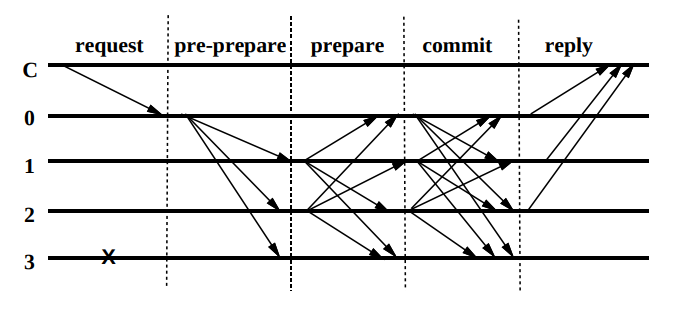
\includegraphics[width=1\linewidth]{PBFT.png}
 	\caption {روش \lr{PBFT}}
 	\label{fig:PBFT}
 \end{figure}
 
 \par
 در این روش حداکثر تعداد تعداد نود‌هایی که باید خطاکار باشند تا بلوک اشتباهی در زنجیره‌ی قالبی ثبت شود برای 
 $3f + 1$
 نود $f$ نود‌است.
 
\section{اثبات‌های بی‌دانش}
اثبات‌های بی‌دانش اولین بار در سال ۱۹۸۵ 
\cite{GHY}
به عنوان روشی ساخت یک روش رمزنگاری متقارن با کلید عمومی استفاده شد. با پیشرفت تکنولوژی اثبات‌های بی‌دانش،‌ روش‌های جامع اثبات بی‌دانش مانند
\lr{ZK-SNARK} 
\cite{zksnark}
و \lr{ZK-STARK} 
\cite{zkstark}
بوجود آمدند. این روش‌ها توانایی اثبات هر محاسباتی را به صورت بی‌دانش دارند و این موضوع باعث استفاده‌ی آن‌ها در کاربردهای بیشتری شد.
\par
با توجه به این که 
\lr{ZK-SNARK}
، به طور خاص خاص پروتکل پینوکیو
\LTRfootnote{Pinocchio}،
فراگیرترین روش برای ایجاد اثبات‌های بی‌دانش است. تحقیقات زیادی در مورد فاز آماده‌سازی و ایجاد پارامترهای عمومی این مدل انجام شده است. همانطور که قبلا اشاره کردیم ورودی‌های این فاز اگر پس از استفاده‌ی اولیه پاک نشوند می‌توانند برای ایجاد اثبات‌های تقلبی استفاده شوند.
\par
از این تحقیق‌ها می‌توان به روش‌هایی
\cite{znsetup} \cite{multipartyparams}
که تلاش در کاهش نیاز به اعتماد در این فاز می‌کنند اشاره کرد. این روش‌ها باعث می‌شوند که برای لو رفت اطلاعات خطرناک احتیاج به تبانی تمامی اعضای موجود در فاز آماده‌سازی باشد.
\par
از دیگر کارهای در این زمینه می‌توان به تلاش‌هایی برای حذف فاز آماده‌سازی به طور کلی اشاره کرد. این روش‌ با تغییر اساسی در پروتکل و استفاده از چندجمله‌ای‌ها 
\cite{nosetup}
مرحله‌ي آماده‌سازی را حذف می‌کند
 
\subsubsection{پروتکل‌های مبتنی بر اثبات‌ بی‌دانش}
از این تحقیقات می‌توان به بستر 
\lr{HAWK}
\cite{hawk}
اشاره کرد. در این تحقیق به کمک یک تعریف کلی از زنجیره‌ی قالبی به عنوان سامانه که همواره در دسترس است و هیچ اطلاعات اشتباهی نمی‌پذیرد اما حریم خصوصی را حفظ نمی‌کند یک بستر قرارداد هوشمند ساخته شده است که در آن به ازای کد قرارداد هوشمند، یک کد برای حفظ حریم خصوصی به کمک اثبات‌های بی‌دانش ساخته می‌شود. روش کار این سامانه‌، مبتنی بر ایجاد آدرس‌های مقصد یکتا به ازای هر تراکنش است. 
\\
مونرو 
\LTRfootnote{Monero}
که یک ارز دیجیتال است که بر اساس الگوریتم 
\lr{Cryptonote}
\cite{monero}
کار می‌کند، به مانند 
\lr{HAWK}
با یکتا سازی آدرس‌های مقصد و امضای حلقه‌ای 
\LTRfootnote{ًRing Signature}
کار می‌کند. در ادامه این ارز دیجیتال با همین روش مدلی 
\cite{monero2}
برای مخفی کردن پرداخت‌کننده‌ی سکه نیز ارائه کرد.
\par
از کارهای دیگر در این زمینه‌ می‌توان به 
\lr{zerocoin}
\cite{zerocoin}
که روش پرداخت ناشناس بر بستر بیت‌کوین به کمک 
\lr{ZK-SNARK}
ارائه کرد اشاره کرد. روش استفاده شده در آن با بهبود در ارز دیجیتال 
\lr{z-cash}
\cite{zerocash}
استفاده شد. این ارز دیجیتال دو مدل سکه‌ی قابل ردگیری و غیرقابل ردگیری دارد و هر کسی می‌توان طی یک تراکنش سکه‌های خود را به سکه‌های ناشناس تبدیل کند.



\cchapter{روش پیشنهادی}
در این بخش یک روش برای رأی‌گیری الکترونیک توزیع‌شده و مبتنی بر زنجیره‌ی قالبی ارائه می‌شود. در این روش برخلاف تلاش‌های مشابه برای ایجاد روش‌های رأی‌گیری امن، ناشناسی رأیء به صورت کامل حفظ می‌شود. برای حل این مسئله به دو پروتکل امن نیاز داریم:یکی بین کاربر و حوزه‌ی رأی‌گیری و دیگری برای به اشتراک‌گذاری اطلاعات بین حوزه‌ها. شکل \ref{fig:toplevel} شمای منطقی سامانه را نشان می‌دهد، دو پروتکل ارائه شده با استفاده از زنجیره‌ی قالبی، نیاز به یک شخص مورد اعتماد را در رأی‌گیری حذف می‌کنند.
\begin{figure}[h!]
	\centering
	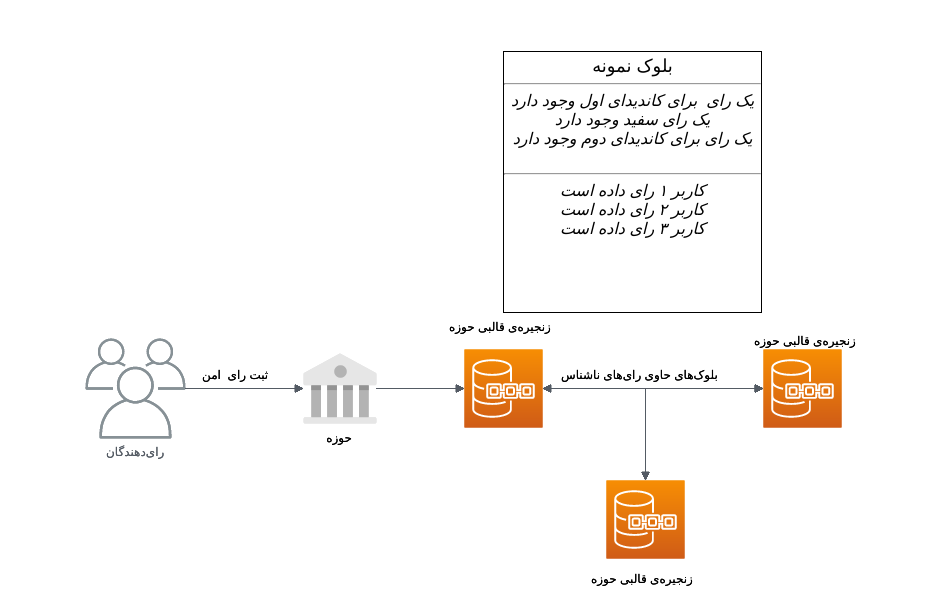
\includegraphics[width=1\linewidth]{toplevel.png}
	\caption {شمای منطقی سامانه}
	\label{fig:toplevel}
\end{figure}


\par
روش پیشنهادی ما سه هدف کلی دارد: ۱- هر رأی‌دهنده از شمارش درست رأی خود اطمینان حاصل کند ۲- حریم خصوصی حفظ شود ۳- هر خطا در فرایند رأی‌گیری قابل تشخیص باشد. برای رسیدن به این اهداف باید فرایند به گونه‌ای طراحی شود که هیچ فردی معتمد فرض نشود. برای این کار ابتدا شرایط و مفروضات مسئله را به طور دقیق‌تر بررسی می‌کنیم، در ادامه روش رأی‌گیری را به صورت کلی و بدون در نظر گرفتن توزیع‌شده بودن سامانه ارائه می‌کنیم و در نهایت با استفاده از یک روش توافق مناسب امنیت پروتکل در حالت توزیع شده را فراهم می‌کنیم. 
\section{تعریف نقش‌ها}
در این بخش نقش‌های حاضر در روش رأی‌گیری و انتظارات خود از آن‌ها را تعریف می‌کنیم:
\begin{itemize}
	\item
	\textbf{ناظر انتخابات}:
	این سازمان مسئول بررسی صحت انتخابات و احراز هویت شرکت‌کنندگان در انتخابات است. به این سازمان فقط در حوزه‌ی احراز هویت اعتماد می‌شود. همچنین این سازمان بررسی‌کننده‌ی نهایی درست بودن انتخابات است و باید بتواند از آن اطمینان حاصل کند.
	\item
	\textbf{رأی‌دهنده}:
	فردی که حق رأی به یک کاندیدا را دارد، این فرد اختیار استفاده کردن یا نکردن از رأی خو را داشته و می‌تواند تلاش کند که چند بار رأی‌دهد. باید بتواند از درستی انتخابات اطمینان حاصل کند زیرا ممکن است توسط یک رقیب بدخواه برای رأی‌دادن تحت فشار قرار بگیرد.
	\item
	\textbf{حوزه‌ی انتخابات}:
	محلی که در آن رأی داده می‌شود، باید به گونه‌ای باشد که امنیت فیزیکی افراد را تامین کند. در عین حال ممکن است برای خراب کردن انتخابات یا نقض حریم خصوصی کاربران تلاش کند. 
\end{itemize}
\section{شرایط مسئله‌ی رأی‌گیری الکترونیک}
شروط لازم برای روش‌ رأی‌گیری ارائه شده عبارت‌اند از:  
\begin{enumerate}
	\item 
	هر فرد واجد شرایط دقیقا یک بار بتواند رأی دهد.
	\item 
	هیچ کسی نتواند به جای فرد دیگری رأی دهد.
	\item 
	هیچ فردی مجبور به رأی دادن نشود.
	\item 
	هیچ فردی مجبور به رأی دادن به کاندیدای خاصی نشود.
	\item 
	در صورت نقض حریم خصوصی و یا شمرده نشدن بعضی رأی‌ها ناظر انتخابات بتواند حوزه‌ی متخلف را شناسایی کند. حوزه‌ها به دلیل در اختیار داشتن سامانه‌های کامپیوتری رأی‌گیری همواره می‌توانند با روش‌های 
	\lr{phishing}
	و یا استفاده از بد‌افزار‌ها حریم خصوصی کاربر را نقض کنند یا رأی او را ثبت نکنند. لذا از آنجا که قابل پیگیری بودن تخلفات حوزه‌ها یکی از مهم‌ترین شرایط یک انتخابات درست است، در صورت خطای حوزه، حوزه‌ی خطاکار باید مشخص شود.
	\item 
	هر رأی‌دهنده بتواند به کمک ابزارهای رمزنگاری اطمینان حاصل کند که رأی او شمرده شده است. این شرط به این معنی است که هر کاربری که دانش کافی داشته باشد باید بتواند از درستی انتخابات - بدون نیاز به اعتماد به حوزه یا حتی ناظر انتخابات - اطمینان حاصل کند. 
	\item
	رأی‌دهنده نیازی به دانش یا توانایی خاصی برای رأی‌دادن نداشته باشد. این نیازمندی برای حفظ دسترس‌پذیری انتخابات لازم است.
	\item
	سامانه رأی‌گیری نسبت به روش‌های فعلی رأی‌گیری از دید کاربر تفاوت چندانی نداشته باشد. هر تغییر اساسی از نگاه رأی‌هنده باعث سختی نسبی انتخابات خواهد شد و هزینه‌ی  استفاده از این روش انتخاباتی را به شدت افزایش خواهد داد.
	\item 
	بتوان نتایج انتخابات را در بازه‌های زمانی معین دید. هر سامانه‌ی انتخاباتی که نتایج را به صورت لحظه‌ای نشان دهد همواره در خطر حمله‌های مبتنی بر زمان در رابطه با حریم خصوصی رأی‌دهندگان خواهد بود، به همین منظور نتایج انتخابات را می‌توان در بازه‌های زمانی که حریم خصوصی را به خطر نیندازد نشان داد.
	\item 
	بتوان از شمرده شدن تمامی رأیء بعد از انتخابات اطمینان حاصل کرد. به دلیل الزام مخفی نگه‌داشتن زمان حدودی ارسال هر رأی، نتایج نهایی انتخابات تنها بعد از اتمام رأی‌گیری قابل اتکاست.
\end{enumerate}

\section{مفروضات مسئله}
مسئله‌ی شناسایی یک مسئله‌ی مهم در هر انتخابات است، با توجه به این که افراد واجد شرایط بسته به هر انتخابات تغییر می‌کنند در این مسئله فرض می‌کنیم که هر رأی‌دهنده یک جفت کلید خصوصی و عمومی دارد که قبل از فرایند انتخابات توسط ناظر انتخابات تایید شده است. 
\par
وظیفه‌ی حفظ امنیت کلید عمومی و خصوصی هر کاربر به عهده‌ی خود کاربر خواهد بود چرا که نشانگر هویت کاربر در سامانه‌ کلید عمومی او خواهد بود. هر چند که برای رأی دادن در حوزه اطلاعات شناسایی کاربر با کلید عمومی او تطابق داده خواهد شد.
\par
هر رأی‌دهنده برای ثبت رأی نیاز به یک دستگاه هوشمند دارد، از آن‌جایی که این دستگاه صرفا برای امضای کورکورانه استفاده می‌شود برای دسترس‌پذیری بالاتر می‌توان این دستگاه را در حوزه ارائه کرد تا رأی‌دهندگان تنها کلید خصوصی خود را در آن وارد کنند.  انجام این کار نیاز اعتماد به حوزه را بالاتر می‌برد چرا که رأی‌دهنده راهی برای اطمینان حاصل کردن از این که دستگاه برنامه‌ی درستی را اجرا می‌کند ندارد.
\par 
هر حوزه یک جفت کلید عمومی و خصوصی دارد که برای امضا کردن بلوک‌های زنجیره‌ی قالبی استفاده می‌شود، همه‌ی حوزه‌ها و ناظر انتخابات قبل از رأی‌گیری از طریق یک کانال امن کلیدهای عمومی خود را به اشتراک می‌گذارند در نتیجه هر حوزه و ناظر انتخابات کلید عمومی تمامی حوزه‌ها را می‌شناسد.

\section{پروتکل ثبت رأی‌}
\subsection{مثال شهودی}
برای به‌دست آوردن دید کلی در راه‌حل ابتدا یک مثال شهودی از یک مدل رأی‌گیری متمرکز را بررسی می‌کنیم،‌ سپس در ادامه از این روش برای ایجاد سامانه‌ی توزیع‌شده و الکترونیک خود استفاده می‌کنیم. به طور کلی این روش مانند شکل \ref{fig:pen} عمل می‌کند.
\begin{figure}[h!]
	\centering
	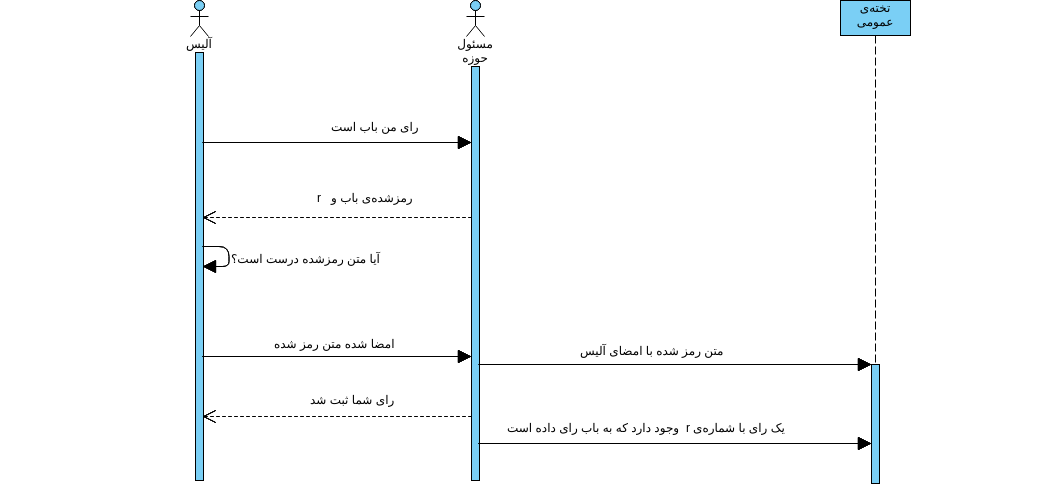
\includegraphics[width=1\linewidth]{penandpaper.png}
	\caption {شمای شهودی}
	\label{fig:pen}
\end{figure}


\par
فرض می‌کنیم در یک رأی‌گیری به ازای هر رأی‌دهنده یک کاغذ نام رأی‌دهنده، یک برگه‌ی رأی و همچنین یک صندوق به ازای هر کاندیدا وجود دارد و همه‌ی این اطلاعات در معرض دید عموم هستند. 
\par
آلیس برای رأی‌دادن یکی از کاندیداها را انتخاب می‌کند، مسئول حوزه یک کاغذ رمز شده که در آن یک شماره‌ی تصادفی $r$ و کاندیدای موردنظر آلیس، باب، نوشته شده را به آلیس می‌دهد تا امضا کند، آلیس پس از اطمینان حاصل کردن از درستی ثبت کاندیدا (ولی بدون فهمیدن $r$) آن را امضا می‌کند. ثبت مسئول حوزه این عبارت رمز شده و برگه‌ی رأی مربوط به آلیس را به تخته می‌چسباند. این فرایند را ثبت رأی‌ می‌نامیم.
\\
در ادامه پس از مدتی مسئول حوزه تخته مراجعه‌ می‌کند و شاهدی بر تخته ثبت می‌کند که ثابت می‌کند او کلید رمزی می‌داند که یکی از کاغذ‌های روی تخته را باز می‌کند که نتیجه‌ی آن $r$ و باب است. سپس یکی از رأی‌های روی تخته را برمی‌دارد و به صندوق باب می‌اندازد. این فرایند را شمارش رأی‌ می‌نامیم.
\par
از آن‌جایی که شاهد ارائه شده یک شاهد بی‌دانش خواهد بود هیچ راهی برای فهمیدن این موضع که شاهد برای رأی آلیس ساخته شده وجود ندارد. حتی خود آلیس چون عدد $r$ را به صورت رمز شده دریافت کرده است، نمی‌تواند شاهد مربوط به خود را پیدا کند. پس می‌دانیم که حریم خصوصی آلیس حفظ شده است. 
\\
 شاهد آلیس در تخته ثبت شده و دیگر نمی‌توان اثباتی ارائه کرد که رأی آلیس را دو بار بشمرد، چرا که عدد $r$ آن تکراری خواهد بود.
\\
چون پلیس یا نظران انتخابات امنیت فیزیکی رأی‌دهنده در محل رأی‌گیری را تضمین می‌کنند، راهی برای مجبور کردن آلیس به رأی دادن به کاندیدای خاصی نخواهد بود و با اضافه کردن صندوق رأی ممتنع می‌توانیم اطمینان حاصل کنیم که کسی آلیس را مجبور به رأی‌دادن نیز نکرده است. 
\par 
تنها مسئله‌ای که به ظاهر حل نشده، این است که آلیس چون یک عبارت رمز شده دریافت کرده نمی‌تواند از درست شمرده شدن رأی خود مطمئن شود، برای حل این مسئله از امضای کورکورانه استفاده کرده‌ایم. این روش به آلیس اجازه می‌دهد که بدون فهمیدن $r$ مطمئن شود که داخل متن رمز شده باب نوشته شده‌است. 
\par 
در انتهای این فرایند تعداد رأی‌ موجود در صندوق باب، تعداد رأی‌های او خواهد بود.
\par 
لازم به ذکر است که در پیاده‌سازی واقعی تخته را با یک زنجیره‌ی قالبی مدل می‌کنیم و مسئول حوزه برنامه‌ی در حال اجرا در حوزه‌ خواهد بود. همچنین صندوق و برگه‌ها‌ی رأی نیز به طور شفاف به عنوان حساب‌هایی در زنجیره‌ی قالبی  محسوب می‌شوند. 


\subsection{فرایند رأی‌گیری از نگاه کاربر}
یکی از مهم‌ترین جنبه‌های طراحی یک سامانه‌ی رأی‌گیری تاثیر آن بر رأی‌دهنده است چرا که در انتخابات‌های بزرگ هزینه‌ی تغییر رفتار رأی‌دهندگان یا سخت‌تر شدن فرایند رأی‌گیری به هر نحوی می‌تواند باعث کاهش شرکت رأی‌دهندگان و افزایش هزینه‌ی تغییر رأی‌گیری شود.
\par
در بعضی روش‌های رأی‌گیری مانند \lr{Follow my vote} کاربر رأی‌دهنده به دسترسی اینترنت نیاز دارد و یا در بعضی روش‌ روش وت‌بوک کاربر باید محل رأی‌دادن خود را پیش از انتخابات تعیین کند. این تغییرات در انتخابات‌هایی با مقیاس بزرگ قابل قبول نیستند. در روش ما کاربر جدا از مرحله‌ی شناسایی اولیه که می‌تواند یک بار به ازای چندین انتخابات انجام شود نیازمند تغییری در رفتار خود نیست. 
\par
برای تشریح فرآیند رأی‌ دادن کاربر، آن را به دو بخش قبل از رأی‌گیری و در حوزه‌ی رأی‌گیری تقسیم می‌کنیم. 
\subsubsection{قبل از رأی‌گیری}
قبل از رأی‌گیری هر فرد واجد شرایط باید از یک روش امن از ناظر انتخابات یک جفت کلید عمومی و خصوصی دریافت کند و یا کلید عمومی خود را در سامانه‌ی مربوط ثبت کند. این کلید می‌تواند در قالب یک فایل بر روی یک دستگاه هوشمند - مثلا تلفن همراه یا حتی یک کارت هوشمند - باشد. این مرحله  می‌تواند در هر انتخابات تکرار شود یا یک فرایند ابتدایی باشد و برای انتخابات‌های بعدی نیز استفاده شود. 
\subsubsection{در حوزه‌ی رأی‌گیری}
در حوزه‌ی رأی‌گیری رأی‌دهنده پس از ورود کارت شناسایی و کلید عمومی خود را ارائه می‌کند، در صورت تایید اطلاعات، کاربر با دستگاه هوشمند خود به سامانه‌ حوزه متصل می‌شود، رأی‌ خود را از بین‌ کاندیدا‌های ممکن و یا ممتنع وارد کرده و پیام تایید را دریافت می‌کند. 
\subsection{فرایند رأی‌گیری از دید حوزه‌}
در این بخش فرایند رأی‌گیری را از نگاه حوزه‌ بررسی می‌کنیم اما صرفا منطق پروتکل را مورد بررسی قرار می‌دهیم و جزییات زنجیره‌ی قالبی و عملیات توزیع شده نمی‌پردازیم. 
\\
برای ثبت رأی یک‌ نفر در ابتدا آن فرد با کارت شناسایی احراز هویت شده و از طریق ارتباط با ناظر انتخابات درستی کلید عمومی آن فرد بررسی می‌شود. در مرحله‌ی بعدی با ارائه‌ی کلید خصوصی کاربر یک تراکنش ثبت با نتیجه‌ی مورد نظر ایجاد می‌کند و تراکنش ثبت توسط دستگاه هوشمند کاربر کوکورانه امضا می‌شود. در این مرحله تراکنش شمارش نیز ایجاد شده و با تاخیر زمانی در زنجیره‌ی قالبی ذخیره می‌شود.

\subsubsection{تراکنش‌ها}
در این بخش تراکنش‌های ثبت و شمارش را تعریف می‌کنیم:
\par
در تراکنش ثبت، یک رأی از یک کلید عمومی به دسته‌ی رأی‌های منتظر شمارش منتقل می‌شود. هر تراکنش ثبت شامل یک رأی و یک رشته‌ی 
\LTRfootnote{string}
رمزشده است که حاوی یک عدد تصادفی $s$ و حساب مقصد $d$ بوده و با کلید تصادفی $k$ رمز شده است. این عبارت رمز‌شده را $CM$ می‌نامیم. سپس $CM$ (نه خود $s$) در زنجیره‌ی قالبی به همراه رأی ثبت می‌شود
\RTLfootnote{لازم به ذکر است که $CM$ بعد از امضا شدن با کلید خصوصی کاربر در زنجیره‌ی قالبی ذخیره می‌شود.}.
\\
\begin{equation}
CM = enc_{k} (r, d)
\label{eq:enc}
\end{equation}

\begin{figure}[h!]
	\centering
	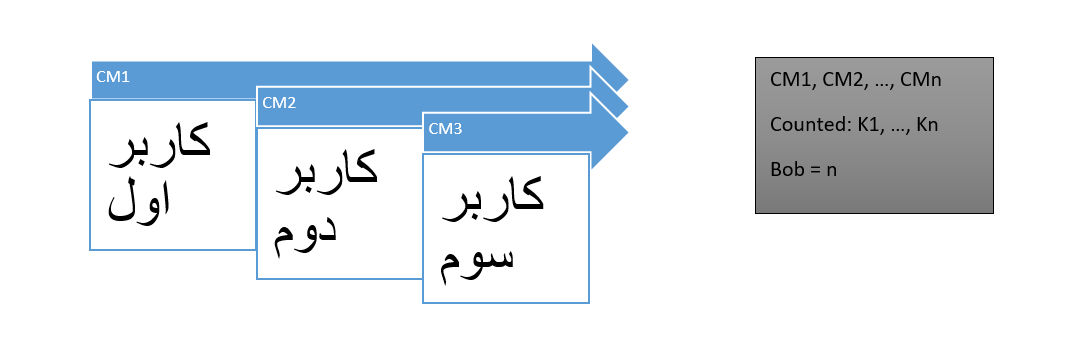
\includegraphics[width=1\linewidth]{commit.PNG}
	\caption {تراکنش ثبت}
	\label{fig:commit}
\end{figure}

\par
تراکنش دیگر تراکنش شمارش است که در آن شاهدی برای شمارش رأی ارائه می‌شود. برای این تراکنش رأی‌دهنده اثباتی بی‌دانش برای دو موضوع ارائه می‌کند: یک $C$ می‌شناسد به طوری که  $C \in C_1, C_2, ... ,C_n$ و یک رشته‌ای $r$ می‌داند که $C$ را به $s$ و $d$ باز می‌کند. در نتیجه‌ی این اثبات یکی از رأی‌های ثبت‌شده به $d$ منتقل می‌شود. 

\begin{figure}[t]
	\centering
	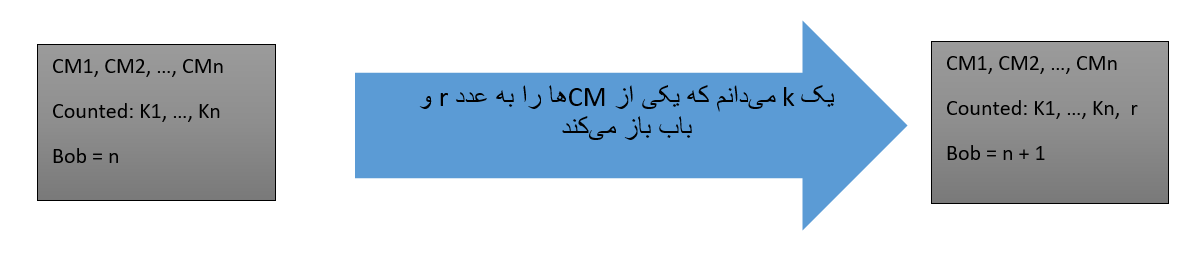
\includegraphics[width=1\linewidth]{Count.PNG}
	\caption {تراکنش شمارش}
	\label{fig:count}
	\end{figure}
\par
برای تحلیل امنیت این روش یک بلوک را تصور می‌کنیم که دارای $n$ تراکنش ثبت و به همین تعداد تراکنش شمارش است و می‌خواهیم از درستی شمارش آگاه شویم. هر تراکنش شمارش یک شاهد بی‌دانش ثبت کرده است که نشان می‌دهد در آن بلوک یک $C_i$ وجود دارد که شماره‌ی آن $r_i$ است. با توجه به این که هر کسی می‌تواند شاهد‌ها را بررسی کند می‌دانیم که هر شاهد ثبت شده درست است. چون رأی‌‌ها در تراکنش ثبت، رمزشده نگهداری می‌شوند برای یافتن رأی‌دهنده‌ی هر شاهد راهی وجود ندارد و با توجه به تکراری نبودن $r$ها می‌دانیم که هیچ رأی دوبار شمرده نشده است. 

\subsubsection{فرایند ثبت رأی کاربر}
در این بخش پروتکل ثبت رأی حوزه را به طور دقیق بررسی می‌کنیم. 

\begin{enumerate}
	\item 
	کاربر گزینه‌ی مورد نظر خود را انتخاب می‌کند، حوزه به تعداد $n$ تا $CM$ می‌سازد که رأی کاربر به کاندیدای مورد نظر را نشان می‌دهند، هر کدام را با یک کلید تصادفی رمز می‌کند و برای تایید به کاربر می‌دهد. 
	\item 
	یکی از از عبارات رمزشده به طور تصادفی توسط کاربر $CM_c$ انتخاب می‌شود و به حوزه اعلام می‌شود.
	\item 
	حوزه کلید مربوط به تمامی $CM$های دیگر را به کاربر ارائه می‌کند.
	\item 
	دستگاه هوشمند کاربر همه‌ی $CM$ها را باز کرده و ثبت رأی‌ها به نام کاندیدای مورد نظر را بررسی می‌کند. با این روش کاربر با احتمال $\frac{n-1}{n}$ از درستی رأی در $CM_c$ مطمئن می‌شود. سپس $CM_c$ را با کلید خصوصی خود امضا می‌کند و به حوزه می‌دهد. در نتیجه‌ امکان فهمیدن عدد تصادفی در $CM_c$، که آن را $s$ می‌نامیم، برای او وجود نخواهد داشت. پاسخ کاربر به شکل \ref{eq:sign} خواهد بود.
	\begin{equation}
	SignedCM = sign_{Priv_{user}} (CM)
	\label{eq:sign}
	\end{equation}
	
	\item
	حوزه، $CM_c$ را به همراه رأی موجود در حساب کاربر به عنوان یک تراکنش ثبت در زنجیره‌ی قالبی ذخیره می‌کند. در صورتی که رأی کاربر قبلا ثبت شده باشد در این مرحله خطا رخ می‌دهد و رأی ثبت نمی‌شود. 
	\item
	حوزه یک شاهد برای شمارش رأی کاربر می‌سازد و هر دوی این تراکنش‌ها در بلوک بعدی زنجیره‌ی قالبی ذخیره می‌شوند.
\end{enumerate}
شکل \ref{fig:seqdiag.png} این توالی فرایند را نشان می‌دهد.
\begin{figure}[h!]
	\centering
	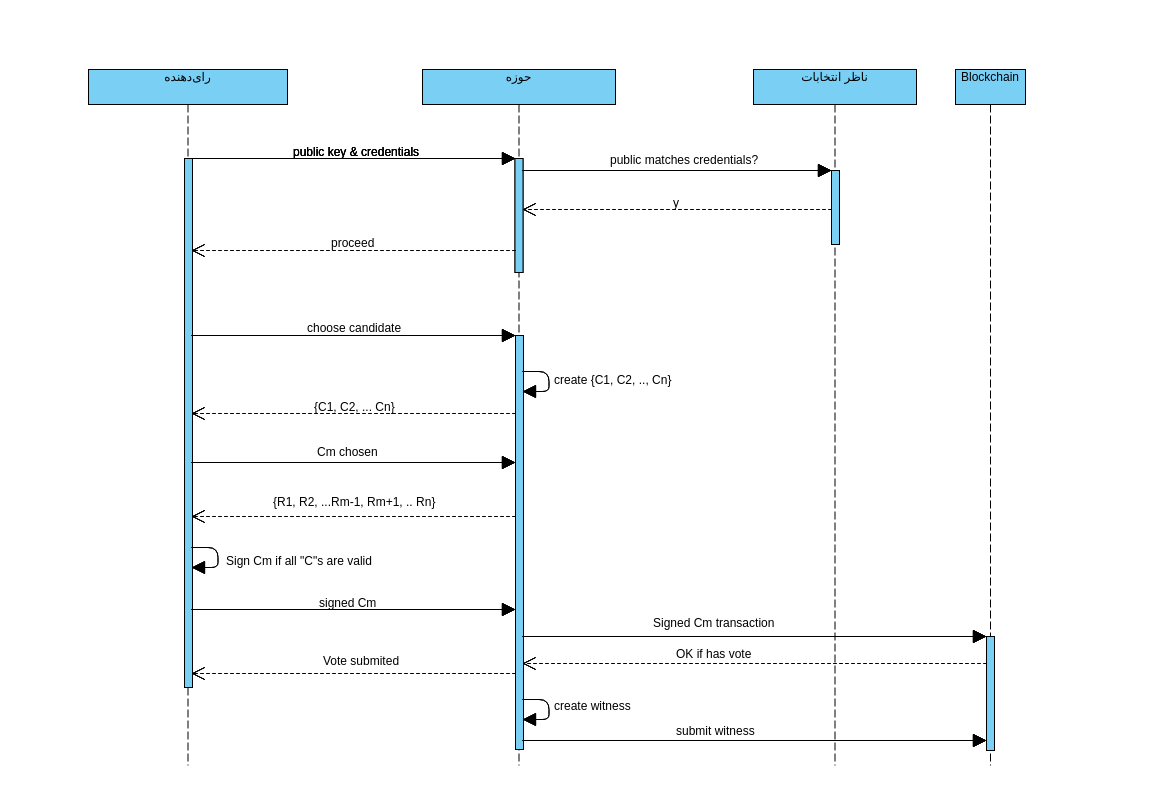
\includegraphics[width=0.9\linewidth]{seqdiag.png}
	\caption {فرایند ثبت رأی در حوزه}
	\label{fig:seqdiag.png}
\end{figure}

\subsubsection{احتمال درستی ثبت رأی}
برای اطمینان از درستی ثبت رأی سناریویی را بررسی می‌کنیم که یک حوزه‌ی خطاکار قصد دارد رأی یک کاربر را تغییر دهد. می‌دانیم در فرایند ثبت رأی، حوزه $n$ عدد $CM$ با شماره‌سریال‌های متفاوت تولید می‌کند. با توجه‌ به این که حوزه باید کلید همه‌ی $CM$ها به جز یکی را به کاربر ارائه کند اگر بیش از یکی از پیام‌ها اشتباه باشد کاربر قطعا متوجه می‌شود. پس تنها راه ممکن برای حوزه‌ی خطاکار این است که فقط $CM$ اشتباه بسازد و همراه $n-1$ عدد $CM$ درست به کاربر ارائه کند که در این شرایط احتمال انتخاب شدن $CM$ اشتباه $\frac{n-1}{n}$ خواهد بود. 
\subsubsection{ناشناس بودن رأی‌گیری}
یکی از اهداف اصلی طراحی این پرتوکل حفظ حریم شخصی کاربر، حتی در شرایطی که تمامی اطلاعات او لو رفته باشد، بوده است. این مسئله معادل این است که باب که در رأی‌گیری شرکت کرده بخواهد اثبات کند به یک کاندیدای خاص ، $T$، رأی داده است. اطلاعاتی که باب برای این کار دارد کلید خصوصی خود و تمامی اطلاعات موجود روی زنجیره‌ی قالبی است. 
\par 
می‌دانیم که اطلاعات مربوط موجود در زنجیره‌ی قالبی در قالب تراکنش‌های ثبت به شکل زیر است.
	\begin{equation}
	\begin{matrix}


S = Random serial number\\
D = Chosen candidate\\
r = Random key\\
CommitTransaction = sign_{Priv_{user}} (enc_r(S,D)) \\

	\end{matrix}
\label{eq:commit}
\end{equation}
 و تراکنش‌های شمارش یک اثبات بی‌دانش است که بدون آشکار کردن $r$، عبارت زیر را اثبات می‌کند.
	\begin{equation}
\exists CM \in \{CM_1, CM_2, ..., CM_n\}  \mid dec_r(CM) = (S,D)
\label{eq:a}
\end{equation}


\par 
باب برای این کار از دو روش می‌تواند استفاده کند، یا باید بتواند اثبات کند که در تراکنش ثبت اون $T$ ثبت شده است و یا به روشی تراکنش شمارش مربوط به رأی خود را پیدا کند. ابتدا روش اول را بررسی می‌کنیم: با توجه به این که تراکنش ثبت مربوط به باب با کلید خصوصی او امضا شده است، پیدا کردن آن ساده به نظر می‌رسد. اما با توجه به این که این تراکنش را کورکورانه امضا کرده کلید مربوط $CM_{bob}$ (یعنی $r$) را ندارد. بهترین شانس باب حمله‌ی با دانستن متن
\LTRfootnote{Known-plaintext attack}
 است چرا که می‌داند در متن باید عبارت $T$ نوشته شده باشد ولی با توجه کوتاه بودن عبارت رمزشده پیدا کردن کلید این روش نیز غیرممکن است. 
 \\
 روش دوم پیدا کردن تراکنش شمارش مربوط به رأی باب است. برای این کار به شماره‌سریال مربوط به تراکنش ثبت نیاز دارد که تنها در تراکنش ثبت به صورت رمزشده ذخیره شده پس این روش نیز نیازمند حل روش اول است و قابل اجرا نیست. 
\section{فرایند‌های توزیع‌شده}
در بخش‌های قبل یک پروتکل ثبت رأی‌ را ارائه کردیم. در این قسمت قصد داریم آن را به صورت توزیع‌شده در تعدادی حوزه، بدون ایجاد خطری در ثبت رأی اجرا کنیم. در ادامه شمای کلی سامانه و روش‌ اضافه کردن بلوک به زنجیره‌ی قالبی را نشان داده و در نهایت به نحوه‌ی استفاده از اثبات‌های بی‌دانش در یک محیط توزیع شده می‌پردازیم.
\subsection{شمای کلی}
به طور کلی سامانه از تعدادی حوزه‌ تشکیل می‌شود که روی یک زنجیره‌ی قالبی توافق می‌کنند. همچین هر حوزه ممکن است بلوکی آماده‌شده و در انتظار تایید از بقیه‌ی حوزه‌ها داشته باشد، یا این که بلوکی از حوزه‌ی دیگری گرفته باشد که باید بررسی و امضا کند، شکل \ref{fig:bigpic} شمای کلی درشت‌دانه‌ی سامانه را نشان می‌دهد.
\\
بلوک ابتدایی این زنجیره‌ی قالبی به ازای هر فرد واجد شرایط یک کلید عمومی و یک رأی ‌دارد. همچنین یک آدرس خروجی به ازای هر کاندیدا وجود دارد؛ بدین صورت که تعداد رأی‌هایی که به آن آدرس فرستاده شده باشند رأی‌های آن‌ کاندیداست. 
 
\begin{figure}[th]
	\centering
	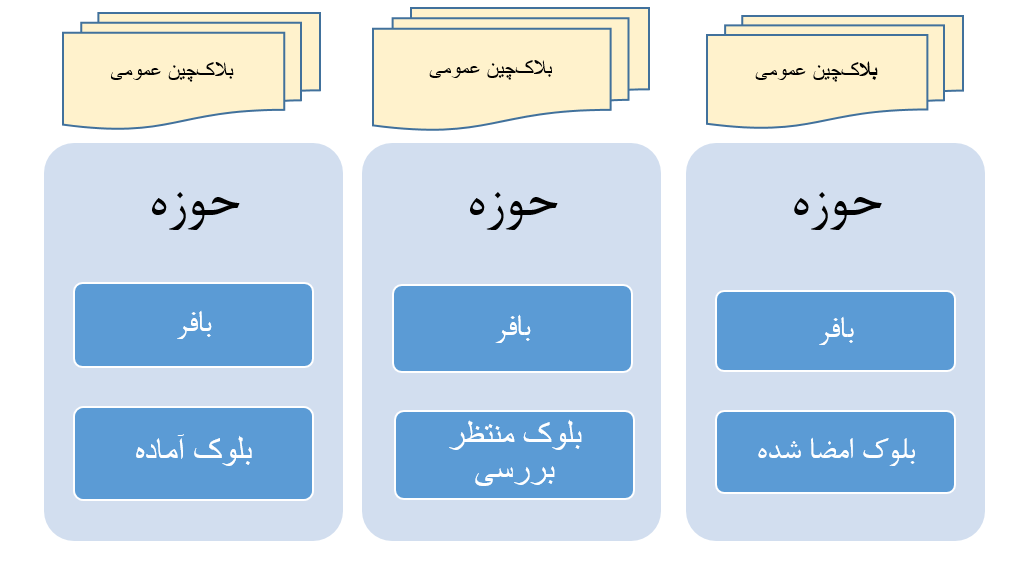
\includegraphics[width=1\linewidth]{blockchain.PNG}
	\caption {شمای منطقی سامانه}
	\label{fig:bigpic}
\end{figure}

\subsection{اضافه شدن بلوک}
می‌دانیم که در هر بلوک ثبت‌شده در زنجیره‌ی قالبی تعدادی از دو مدل تراکنش‌های ثبت و شمارش داریم، همچنین هش بلوک قبلی را نیز برای اطمینان از تغییر نکردن بلوک‌های قبلی نگه ‌می‌داریم. هر حوزه تراکنش‌های ثبت و شمارش خود را دی یک بافر
\LTRfootnote{Buffer}
یا «بلوک پیشنهادی» ثبت و به صورت دوره‌ای برای بررسی و تایید به بقیه‌ی حوزه‌ها ارسال می‌کند. 

\subsection{بررسی بلوک}
هر بلوکی که برای اضافه شدن به زنجیره‌ی قالبی به دست یک حوزه می‌رسد برای درستی بررسی می‌شود. ابتدا باید تک‌‌تک تراکنش‌های ثبت موجود در بلوک توسط رأی‌دهنده‌‌ای که در بلوک‌های قبلی رأی‌ نداده امضا شده باشند. با این بررسی ساده تا زمانی که همه‌ی حوزه‌ها روی یک نسخه از زنجیره‌ی قالبی توافق داشته باشند، هیچ فردی نمی‌تواند دو بار رأی ‌دهد.
\\
همچنین تراکنش‌های شمارش از دو جنبه بررسی می‌شوند: اول درستی اثبات‌ بی‌دانش بررسی می‌شود که شاهد اشتباهی در بلوک وجود نداشته باشد. در مرحله‌ی دوم شماره‌ی سریال‌های موجود در تراکنش‌های شمارش با بلوک‌های قبلی مقایسه می‌شوند تا اطمینان حاصل شود که یک تراکنش شمارش دو بار در زنجیره‌ی قالبی ظاهر نشده است. با این بررسی تا زمانی که تمامی حوزه‌ها روی یک زنجیره‌ی قابلی توافق داشته ‌باشند هیچ رأی دو بار شمرده نخواهد شد.
\par
در نهایت نیز هش بلوک قبلی در بلوک منتظر بررسی با هش آخرین بلوک زنجیره‌ی قالبی مقایسه می‌شود. در صورت تفاوت این دو نیز بلوک رد می‌شود. در صورتی که هر کدام از بررسی‌ها مغایرتی پیدا شود کل بلوک رد می‌شود اما در صورت موفقیت آن‌ها حوزه بلوک پیشنهادی را با امضای دیجیتال خود تایید می‌کند. همانطور که پیش‌تر بررسی کردیم در صورتی که نسخه‌ای یکسان زنجیره‌های قالبی بین حوزه‌ها وجود داشته باشد می‌توانیم از شمارش درست رأی مطمئن شویم. بنابراین به یک روش توافق امن بین حوزه‌ها نیاز داریم.


\subsection{توافق}
برای توافق نیز از روش \lr{PBFT} استفاده می‌کنیم. این روش به ما این امکان را می‌دهد که با در دسترس بودن بیش از یک سوم حوزه‌ها انتخابات را بدون خطر گم شدن بلوک (و در نتیجه رأی)، به درستی اجرا کنیم. با استفاده از این روش در هر زمان یک حوزه‌ی رهبر داریم که می‌تواند بلوکی جدید به زنجیره‌ی قالبی اضافه کند، هر حوزه‌ای که قصد اضافه کردن بلوک جدید را داشته باشد، آن را برای حوزه‌ی رهبر می‌فرستد و رهبر برای بقیه‌ی حوزه‌ها ارسال می‌کند تا بررسی و امضا شود. 

\par 
رهبر در طول زمان تغییر می‌کند و این مسئولیت میان حوزه‌ها در گردش خواهد بود اما با توجه  به این که در هر زمان دقیقا یک رهبر وجود دارد هیچ زمانی دو بلوک متفاوت، توسط حوزه‌ها تایید نمی‌شوند و امکان ایجاد شاخه در زنجیره‌ی قالبی آن‌ها وجود نخواهد داشت. برای تضمین این موضوع که حتی در صورت قطع شدن شبکه‌ی بین حوزه‌ها، دو رهبر هم‌زمان تایید نمی‌شوند، هر حوزه‌ای که ارتباطش با نیمی از حوزه‌های دیگر قطع شود دیگر بلوکی برای تایید ارسال نمی‌کند و رهبر نیز نمی‌شود. این موضوع به این معنی است که ممکن است در بعضی بازه‌های زمانی، یک حوزه‌ی خاص نتواند بلوک خود را ثبت کند و باید رأی‌ها را در بافر خود تا زمانی که ارتباط او با حوزه‌های دیگر متصل شود، نگه‌ دارد.

\cchapter{تحلیل و ارزیابی}
در این فصل به تحلیل و بررسی روش ارائه‌شده و مقایسه‌ی آن با روش‌های دیگر رأی‌گیری می‌پردازیم. همچنین جزئیات پیاده‌سازی تست‌شده در روش، نحوه‌ی ارضای شرایط رأی‌گیری ایده‌آل، این روش را در قیاس با روش‌های دیگر از نظر هزینه و میزان اعتماد مورد نیاز بررسی می‌کنیم. 
\par
لازم به ذکر است که هدف این تحقیق ارائه‌ی یک پروتکل رأی‌گیری امن است لذا در این روش به سرعت اجرا در یک محصول کامل نمی‌پردازیم. برای مثال برای بهینه‌سازی حجم شاهد‌های بی‌دانش در محیط واقعی باید از تجمیع‌گر‌های یک طرفه 
\LTRfootnote{One-way accumulator}
که اولین بار در سال ۱۹۹۳ 
\cite{oneway}
ارائه شدند و یا روش‌های مشابه استفاده کرد. این روش‌ها در پروتکل‌های مشابه مانند زی‌کش در مقیاس بزرگ استفاده‌ شده‌اند و می‌دانیم که مسئله‌ی سرعت و مقیاس‌پذیری چالشی بزرگی در استفاده از این محصول نخواهد بود.

\section{پیاده‌سازی}

در پیاده‌سازی این کار به ابزاری برای ایجاد یک زنجیره‌ی قالبی خصوصی با روش توافق \lr{PBFT} نیاز داریم لذا از 
\lr{hyperledger fabric} \LTRfootnote{https://www.hyperledger.org/projects/fabric}
که یک بستر قراردادهای هوشمند است استفاده شده است. 
\lr{hyperledger fabric}
توسط شرکت \lr{IBM} طراحی شده و توسط \lr{Linux Foundation} نگهداری می‌شود. این پروژه یک زنجیره‌ی قالبی خصوصی ارائه می‌کند که قسمت‌های مختلف آن مانند روش توافق به سادگی قابل تغییرند. این ابزار که به کمک \lr{NodeJS} نوشته شده است، به کمک داکر 
\LTRfootnote{Docker}
به سادگی تعدادی نود با یک بلاک‌چین خصوصی ایجاد می‌کند. همچنین به کمک نوشتن قرارداد‌های هوشمند بر روی این بستر حوزه‌های مورد نیاز را ایجاد کردیم.
\par 
مسئله‌ی بعدی روش ایجاد اثبات‌های بی‌دانش است که برای ایجاد تراکنش‌های شمارش نیاز به آن‌ها داریم. برای ساخت اثبات‌های بی‌دانش از کتابخانه‌ی 
\lr{libsnark}\LTRfootnote{https://github.com/scipr-lab/libsnark}
استفاده شده است که الگوریتم پینوکیو را با زبان \lr{C++} پیاده کرده است . \lr{Zcash} - یکی از بزرگ‌ترین ارز‌های دیجیتال با توانایی تراکنش ناشناس - نیز برای ساخت اثبات از این کتابخانه استفاده کرده است.
\par
همانطور که قبلا اشاره کردیم برای استفاده از روش \lr{ZK-SNARK} برای ایجاد‌ شاهد‌های بی‌دانش به توافق روی نقاط اولیه‌ای روی یک \lr{elliptic curve} نیاز داریم. در کتابخانه‌ی \lr{libsnark} برای انجام این کار از روش ارائه شده در تحقیق 
\cite{multipartyparams}
استفاده شده است. برای این کار حوزه‌ها در یک زنجیره چیده می‌شوند و هر کدام قسمتی از محاسبات لازم برای ایجاد نقطه‌های اولیه را انجام می‌دهند، به صورتی که حتی با حذف یکی از آن‌ها نیز محاسابات ناتمام بماند. سپس با یک حالت خاص از اثبات‌های بی‌دانش انجام محاسبات را به یکدیگر اثبات می‌کنند. با این روش برای دسترسی به نقاط اولیه برای ایجاد شاهد‌های تقلبی، به نتیجه‌ی محاسبات تمامی حوزه‌ها نیاز داریم؛ به عبارت دیگر برای ایجاد شاهد‌های تقلبی، تمامی حوزه‌ها باید در فاز آماده‌سازی تبانی کرده و اطلاعات خصوصی خود را به اشتراک بگذارند.
\par 
در فرایند کامپایل این کتابخانه از تنظیمات موجود در جدول \ref{tab:libsnark} استفاده شده است. 
\begin{table}[h!]
	\begin{center}
		%		\def\arraystretch{2}
		\caption{تنظیمات \lr{libsnark}}
		\begin{tabular}{|c|c|c|}
			\hline
			نام متغیر& مقدار & توضیحات \\
			\hline
			CURVE & \lr{ALT\_BN128} & مدل خم مورد استفاده با ۱۲۸ بیت امنیت \\
			\hline
			MULTICORE & ON & استفاده از چند هسته برای موازی سازی \\
			\hline
			USE\_PT\_COMPRESSION & OFF & سرعت بالاتر در ازای حجم شاهدهای بزرگتر \\
			\hline
			PROFILE\_OP\_COUNTS & OFF & شمارش تعداد فعالیت روی خم 
			 \\
			 \hline
		\end{tabular}
		\label{tab:libsnark}
	\end{center}
\end{table}
\\
بقیه‌ی تنظیمات کتا‌بخانه در حالت پیش‌فرض استفاده شده است.
\section{معیار‌های رأی‌گیری مناسب}
یک روش رأی‌گیری خوب باید  شروط رأی‌گیری ایده‌آل را داشته باشد. شروط ارائه‌شده نیازمندی‌های اصلی یک رأی‌گیری هستند و در صورت اجرا نشدن آن‌ها، روش رأی‌گیری در کاربرد‌های مهم و بزرگ قابل استفاده نیست. 
\par 
از آنجا که در رأی‌گیری‌های مهم، برنده شدن در انتخابات می‌تواند سود بسیار زیادی برای یک کاندیدا داشته باشد همواره انگیزه برای هزینه کردن برای تخلف در انتخابات وجود دارد. لذا برای اطمینان از یک انتخابات امن باید نیاز اعتماد به افراد به حداقل برسد و هر گونه تخلف قابل ردیابی باشد. 
\par 
فاکتور مهم دیگر هزینه‌ی برگزاری انتخابات است.انتخاباتی که امنیت را به خوبی تامین کند ولی هزینه‌ی گزافی برای رأی‌دهنده یا مجری انتخابات داشته باشد، در عمل استفاده نخواهد شد. بنابراین یکی از مهم‌ترین معیارهای ارزیابی روش رأی‌گیری، هزینه‌ی آن است. 
\par 
مسئله‌ای دیگر که در هر سامانه‌ی توزیع‌شده‌ای به بررسی دقیق نیاز دارد، نحوه‌ی نگهداری داده‌هاست. در این سامانه‌ها به دلیل مشکلات ذاتی شبکه از قبیل گم شدن پیام و یا تأخیر در رسیدن پیام‌ها، همواره احتمال ایجاد ناهمخوانی بین داده‌های قسمت‌های مختلف شبکه وجود دارد. به همین دلیل در بخش پایانی این فصل به بررسی روش توافق استفاده شده در این راه‌حل و تاثیر آن در همخوان نگه‌داشتن اطلاعات حوزه‌ها می‌پردازیم. 
\par
به دلیل اهمیت بالای نیازمندی‌های رأی‌گیری ایده‌آل، ابتدا نشان می‌دهیم که روش پیشنهادی این تحقیق چگونه هر کدام از این نیازمندی‌ها را برطرف می‌کند سپس در ادامه با مقایسه‌ی آن با تحقیقات دیگری که توانسته‌اند این شروط را رعایت کنند نحوه‌ی اطمینان شمارش درست، خطر از بین رفتن ناشناسی رأی‌ها، هزینه‌ی برگزاری، هزینه‌ی تغییر برای کاربر و در نهایت توانایی پیدا کردن خطاهای حوزه‌ها را بررسی می‌کنیم.
\section{شباهت به رأی‌گیری ایده‌آل}
در این بخش نیازمندی‌های رأی‌گیری ایده‌آل را دوره می‌کنیم تا مشخص شود که روش ارائه شده چگونه هر کدام از نیاز‌مندی‌ها را رفع می‌کند.

\begin{itemize}
	\item 
	می‌دانیم که هر شخصی حداکثر می‌تواند یک رأی‌ بدهد؛ زیرا در حساب کلید عمومی آن فرد دقیقا یک رأی در ابتدای رأی‌گیری وجود دارد. از طرفی سامانه مانع رأی دادن او نمی‌شود چرا که رأی‌دهنده می‌تواند مصرف شدن رأی خود را در زنجیره‌ی قالبی بررسی کند.
	\item 
	می‌دانیم کسی نمی‌تواند به جای دیگری رأی دهد، چرا که برای رأی دادن هم به دسترسی به کلیدخصوصی نیاز دارد و هم کلید عمومی فرد با اطلاعات شناسایی او در حوزه مقایسه می‌شود.
	\item 
	با اضافه شدن گزینه‌ی ممتنع و حفظ امنیت فیزیکی حوزه‌ی رأی‌گیری می‌توانیم اطمینان حاصل کنیم که کسی مجبور به رأی‌ دادن نمی‌شود.
	\item 
 هیچ کسی مجبور به رأی‌دادن به شخصی خاص نمی‌شود چرا که راهی برای بررسی رأی‌ فرد بعد از فرایند رأی‌گیری وجود ندارد، در نتیجه به دلیل امن بودن حوزه‌ی رأی‌گیری، رأی‌دهنده همواره می‌تواند به کاندیدای دلخواه خود رأی‌ دهد و حتی این عمل را انکار کند.
	\item 
	در انتهای انتخابات می‌توانیم به سادگی با بررسی تعداد تراکنش‌های ثبت و شمارش، از درستی شمارش رأی اطمینان حاصل کنیم. هر شخص نیز با بررسی این که عمل ثبتی برای او در زنجیره‌ی قالبی وجود دارد می‌تواند از شمرده شدن رأی خود مطمئن شود.
	\item 
	از آن جا که تراکنش‌های ثبت کورکورانه امضا می‌شوند، نتیجه‌ی رأی ناشناس باقی می‌ماند؛ حتی خود رأی‌دهنده با وجود اطمینان از نتیجه‌ی رأی راهی برای بررسی نتیجه‌ی برگه‌ی رأی خود را بعد از انتخابات ندارد.
	\item 
	در هر زمانی که یک بلوک جدید در زنجیره‌ی قالبی ثبت شود می‌توان با استناد بر حساب‌های کاندیداها از نتیجه‌ی آن لحظه‌ی انتخابات مطلع شد. همچنین در صورتی که مجری انتخابات نخواهد نتایج لحظه‌ای را منتشر کند می‌تواند زنجیره‌ی قالبی را تا پایان انتخابات بسته نگه دارد. 
\end{itemize}




\section{مقایسه با کارهای مشابه}
در این بخش به مقایسه‌‌ی روش رأی‌گیری ارائه شده با تحقیقات دیگر در این زمینه می‌پردازیم و آن را از چند جنبه‌ی نحوه‌ی اطمینان از ثبت رأی، ناشناسی آرا،  میزان اعتماد مورد نیاز و  هزینه‌ی انتخابات بررسی می‌کنیم. 
\subsection{روش‌های رأی‌گیری دیگر}
برای مقایسه سامانه‌های رأی‌گیری زیر را بررسی می‌کنیم:
\begin{itemize}
	\item 
	\textbf{رأی‌گیری سنتی}:
	این روش به عنوان خط مبنای تحقیق بررسی می‌شود. روش‌های رأی‌گیری الکترونیکی ساخته شده تاکنون، همواره با وجود کاهش هزینه‌ها برای شمارش رأی‌ها، در زمینه‌های امنیت و حریم خصوصی خطرهایی ایجاد کرده‌اند. به همین دلیل رأی‌گیری سنتی همچنان در برخی موارد ممکن است بهتر از روش‌های دیگر عمل کند لذا روش‌های جدید رأی‌گیری باید با این روش مقایسه شوند. نحوه‌ی برگزاری انختابات در این روش در بخش ۱.۲ توصیف شده است. 
	\item \textbf{رأی‌‌گیری الکترونیک بدون زنجیره‌ی قالبی}:
	در این روش، رأی‌گیری الکترونیک متمرکز را بررسی می‌کنیم، چرا که سامانه‌های رأی‌گیری توزیع‌شده‌ی بدون زنجیره‌ی قالبی به کاربرد عمومی نرسیدند. در این سامانه‌ها اطلاعات رأی‌دهندگان و نتیجه‌ی رأی آن‌ها به دلیل نیاز به روش ردگیری به طور کامل ثبت می‌شود اما در فرایند ثبت رأی تفاوت چندانی با سامانه‌های سنتی ندارند.
 	\item \textbf{وت‌بوک}:
 	این روش را به عنوان مصداقی از سامانه‌های رأی‌گیری با زنجیره‌ی قالبی خصوصی بررسی می‌کنیم. 
 	در این روش از یک‌ زنجیره‌ی قالبی - که می‌توان در حالت خصوصی یا عمومی از استفاده کرد - برای ثبت آراء استفاده می‌شود. 
\end{itemize}
\subsubsection{موارد حذف‌شده از مقایسه}
 	 اگرچه روش‌ معروف \lr{VoteWatcher} نیز فعالیت‌های بسیاری در این زمینه داشته، به دلیل عمومی نبودن اطلاعات پیاده‌سازی این سامانه‌، از مقایسه‌ی آن خود‌داری می‌کنیم. 
 	 \\
 	 از آن‌جا که روش‌های رأی‌گیری به کمک یک زنجیره‌ی قالبی عمومی و یا روش‌های توزیع‌شده بدون زنجیره‌ی قالبی به دلیل مشکلات مقیاس‌پذیری توانایی استفاده شدن در انتخابات‌های بزرگ (بیش از چند هزار نفر) را ندارند از بررسی این نوع سامانه‌ها صرف نظر می‌کنیم.
 	 \\
 	 همچنین روش مورد استفاده در \lr{Follow my Vote} از لحاظ روش پیاده‌سازی شباهت زیادی به وت‌بوک دارد ولی در آن به جای حوزه‌ی رأی‌گیری از یک برنامه در رایانه‌ی شخصی یا تلفن هوشمند استفاده می‌شود. اگرچه این روش به سادگی فرایند رأی‌گیری برای بعضی از رأی‌دهندگان کمک می‌کند، دو مشکل بزرگ به همراه دارد که باعث شده از مقایسه‌ی آن خودداری کنیم؛ اولین مشکل کاهش دسترس‌پذیری این روش برای افرادی است که دسترسی به اینترنت ندارند و دومین مشکل انبودن راهیی برای اطمینان از عدم اجبار رأی‌دهنده به کاندیدای خاص به دلیل فقدان حوزه‌ای امن است.
\subsection{هزینه‌ی اطمینان از شمارش درست}
شاید مهم‌ترین شرط برگزاری یک انتخابات میزان اطمینان از شمارش درست آراء در آن‌ باشد. در این بخش به بررسی نحوه‌ی شمارش آراء در روش‌های مختلف می‌پردازیم. 
\par
در روش سنتی برای شمارش آراء بعد از اتمام انتخابات برگه‌های رأی‌ موجود در صندوق‌ها به مکانی منتقل می‌شوند و در آن‌ جا به روش انسانی و یا با استفاده از دستگاه‌های الکترونیکی شمرده می‌شوند. طبیعتا به دلیل دخالت انسانی در این روش شمارش، احتمال خطا زیاد است. همچنین برای اطمینان درستی شمارش یک حوزه، تنها روش شمارش کامل برگه‌های رأی‌ آن حوزه است که هزینه‌ی آن معادل هزینه شمارش اولیه می‌باشد. 
\par 
در روش‌های رأی‌گیری بدون زنجیره‌ی قالبی برای ثبت رأی، اطلاعات کاربر به طور رمزشده به همراه نتیجه‌ی رأی‌ او ثبت می‌شود. دلیل نگه‌داشتن اطلاعات رأی‌دهنده توانایی رد‌گیری و بررسی درستی شمارش آراء است. در این سامانه‌ها شمارش رأی‌گیری به صورت آنلاین صورت می‌گیرد و هزینه‌ی چندانی ندارد، همچنین بررسی ناظر انتخابات هزینه‌ ناچیزی خواهد داشت. 
\par 
روال شمارش در روش پیشنهادی این تحقیق تفاوت چندانی با وت‌بوک ندارد و هزینه‌ی اضافه‌ای برای شمارش آراء اضافه نمی‌کند. اما در این دو روش با عمومی شدن زنجیره‌ی قالبی قبل یا در حین رأی‌گیری رأی‌دهندگان نیز می‌توانند از درستی شمارش آراء و شمرده شدن رأی خود اطمینان حاصل کنند. 
\subsection{حریم خصوصی}
در روش سنتی برگزاری انتخابات با توجه به ناشناس بودن برگه‌های رأی در صندوق رأی‌گیری راهی برای فهمیدن نتیجه‌ی رأی‌ یک فرد خاص نیست. البته با توجه به این که حوزه‌ی رأی‌گیری برگه‌های رأی را از قبل از انتخابات در دسترس دارد، این گزاره در صورتی صحیح است که آن با شماره یا علامت ناشناسی برگه‌های رأی را از بین نبرده باشد.
\par 
در روش‌های رأی‌گیری الکترونیک بدون زنجیره‌ی قالبی، اطلاعات رأی‌گیری با توجه به عمومی نشدن، محفوظ می‌مانند. در این روش نیز حوزه‌ی انتخابات که مسئولیت رمز کردن اطلاعات شخصی کاربر را دارد می‌تواند به حریم خصوصی آسیب بزند. همچنین برای جلوگیری از دو بار رأی دادن یک کاربر باید مرکز مستقلی که اطلاعات رأی‌گیری را ذخیره می‌کند توانایی بازگشایی اطلاعات کاربر را داشته باشد. در نتیجه این مرکز و تمامی افرادی که به اطلاعات آن دسترسی دارند نیز می‌توانند حریم خصوصی را نقض کنند. 
\par
در روش وت‌بوک هر رأی‌دهنده یک «شماره‌ی رأی‌دهنده» دارد و بعد از رأی دادن نیز یک «شماره‌ی رأی» دریافت می‌کند. در ادامه هش شماره‌ی رأی و شماره‌ی رأی‌دهنده در زنجیره‌ی قالبی به عنوان رأی‌دهنده ثبت می‌شود. در این روش علاوه بر حوزه، هر کسی که شماره‌ی رأی و شماره‌ی رأی‌دهنده را داشته باشد می‌تواند از نتیجه‌ی رأی آن فرد آگاه شود. شماره‌های رأی‌دهندگان در یک زنجیره‌ی قالبی خصوصی مستقل نگهداری شده و هیچ وقت عمومی نمی‌شوند. در نتیجه جدا از حوزه‌ی رأی‌گیری فقط خود فرد (یا کسی که اطلاعات خصوصی او را از خودش دریافت کند) می‌تواند نتیجه‌ی رأی فرد را بررسی کند. 
\par 
در روش پیشنهادی ما برای از بین بردن ریسک لو رفتن اطلاعات، درست ثبت شدن رأی در خود حوزه به کاربر اثبات می‌شود و چون او تراکنش ثبت را کورکورانه امضا می‌کند بعد از فرایند ثبت رأی راهی برای پیدا کردن نتیجه‌ی رأی فرد وجود ندارد. در این روش نیز مانند همه‌ی روش‌های ممکن در رأی‌گیری حوزه‌ی خطاکار می‌تواند در حین دریافت رأی نتیجه‌ی آن را جداگانه ثبت کند و از این روش به حریم خصوصی آسیب بزند اما با توجه به این که تمامی بلوک‌ها توسط حوزه‌ها امضا شده‌اند در صورت نقض حریم خصوصی به سادگی حوزه‌ی خطاکار مشخص می‌شود.

\subsection{هزینه‌ی برگزاری}
در این بخش هزینه‌ی برگزاری انتخابات با هر کدام از روش‌ها را از دید کاربر و مجری انتخابات بررسی می‌کنیم.
\subsubsection{هزینه برای کاربر}
فرایند رأی‌دادن کاربر در روش‌هایی که بررسی می‌کنیم به سه حالت خواهد بود:
\begin{itemize}
 \item 
 در روش‌ سنتی و رأی‌گیری بدون زنجیره‌ی قالبی کاربر برای رأی‌دادن صرفا به کارت شناسایی نیاز دارد. او با ارائه‌ی این کارت و بعد از بررسی شدن این که کاربر دو بار رأی نداده رأی خود را ثبت می‌کند. 
 \item 
 در رأی‌گیری با زنجیره‌ی قالبی با هدف افزایش شفافیت و ایجاد اطمینان از شمارش درست آراء برای کاربر، هر کاربر نیاز به ثبت یک «هویت یکتا» در سامانه‌ی مربوط به انتخابات دارد. در وت‌بوک این کار با شماره‌ی رأی‌‌دهنده صورت می‌گیرد و همچنین کاربر باید قبل از رأی‌ دادن حوزه‌ی مد نظر خود را برای رأی ‌دادن مشخص کند. دلیل مشخص کردن حوزه این است که شماره‌ی رأی‌دهندگان از قبل در حوزه ذخیره شده باشند. بنابراین به روال رأی‌گیری کاربر در روش سنتی، یک مرحله‌ی آماده‌سازی اضافه می‌کند که باید در مدت زمان کوتاهی قبل از انتخابات انجام شود، چرا که در رأی‌گیری باید حوزه‌ی رأی‌دهندگان از قبل مشخص شده باشد.
 
 \item
 در سامانه ما نیز کاربر باید قبل از رأی‌گیری یک کلید عمومی برای فرایند رأی‌گیری ثبت کند. همچنین برای اطمینان از درست شمرده شدن رأی خود باید از یک دستگاه هوشمند برای عمل امضای کورکورانه استفاده کند. بنابراین نیاز به این دستگاه نیز به هزینه‌های رأی‌دهنده اضافه می‌شود. 
 \RTLfootnote{
 لازم به ذکر است که کاربر می‌تواند از دستگاه‌های درون حوزه استفاده کند ولی با این کار باید اعتماد کند که حوزه رأی او را به درستی ثبت کرده است چرا که راهی برای اثبات درستی برنامه‌ی موجود در حوزه وجود ندارد.یعنی می‌توان هزینه‌ی کاربر را در فرایند رأی‌گیری کمتر کرد ولی این عمل باعث می‌شود که یک حوزه‌ی خطاکار بتواند رأی کاربر را از طریق حمله‌ی \lr{phishing} تغییر دهد.}
\end{itemize}
\subsubsection{هزینه انتخابات برای مجری}
در روش سنتی انتخابات هزینه‌ی اولیه‌ای برای مجری اعمال نمی‌شود اما در هر انتخابات جدا از هزینه‌ی ایجاد حوزه، هزینه‌ی تولید برگه‌ی رأی فیزیکی و شمارش را باید پرداخت کند. 
\\
در روش‌های رأی‌گیری الکترونیک متمرکز جدا از سامانه‌های کامپیوتری حاضر در حوزه، هزینه‌‌ای به مجری تحمیل نمی‌شود، اما دستگا‌ه‌های الکترونیکی نیازمند بررسی و ارتقا در طول زمان هستند.
\\
در وت‌بوک علاوه بر سامانه‌های موجود در حوزه‌ها، یک سامانه‌ برای ثبت و نگهداری اطلاعات محل رأی‌گیری و شماره‌ی رأی‌دهنده برای هر کاربر وجود دارد که این مسئله نیز نیازمند بررسی امنیتی مداوم و ارتقا بوده و هزینه‌ی نگهداری در طول زمان این روش را افزایش می‌دهد. 
\\
در روش پیشنهادی ما نیز علاوه بر سامانه‌ی موجود در حوزه، مجری انتخابات در هر انتخابات باید توانایی عوض کردن یا ثبت کلید عمومی جدید را به رأی‌دهندگان بدهد که این مسئله هزینه‌ی نگهداری به او اضافه می‌کند. 
\subsection{توانایی ردگیری خطا}
برای درستی انتخابات به یک ناظر انتخابات نیازمندی که بتواند از درستی برگزاری آن اطمینان حاصل کند. با توجه به این که یک حوزه‌ی انتخابات خطاکار همواره می‌تواند بعضی رأی‌ها را شمارش نکند و یا تلاش کند که رأی جعلی تولید کند، در این بخش توانایی ردگیری همچین حملاتی را بررسی می‌کنیم.
در روال سنتی رأی‌گیری با توجه به کاغذی بودن آراء و وصل نبودن برگه‌ی رأی به کاربر، فراتر از بررسی تعداد آراء و مقایسه‌ی آن‌ها با تعداد برگه‌ی ثبت رأی راهی برای بررسی درستی نتایج حوزه وجود ندارد. اگرچه ایجاد برگه‌ رأی‌های غلط هزینه بر است در انتخابات‌های حساس ممکن است به صرفه باشد و در صورت بروز همچین مشکلاتی، راه‌حلی مناسب برای پیدا کردن مشکل وجود ندارد. همچنین در صورتی که بخشی از آراء توسط حوزه دور ریخته شود، ناظر انتخابات هیچ راهی برای فهمیدن آن ندارد و رأی‌دهندگان عادی نیز روش ار شمرده نشدن رأی خود مطلع نخواهند شد.
\par 
در روش‌های رأی‌گیری الکترونیک بدون زنجیره‌ی قالبی  رأی‌دهنده راهی برای اطمینان حاصل کردن رأی‌‌دهنده از شمارش رای خود ندارد. همچنین ناظر انتخابات نیز نمی‌تواند رأی‌هایی را که فرستاده نشده‌اند تشخیص دهد. با توجه به این که حوزه اعلام می‌کند کدام کاربرها در آن رأی داده‌اند، ایجاد رأی دروغین توسط حوزه هم ممکن است. 
\par 
در روش‌ وت‌بوک برای اطمینان از شمارش آراء تمامی رأی‌ها به صورت شفاف ذخیره می‌شوند و هر کسی با اطلاعات شخصی خود می‌تواند درستی ثبت رأی خود را بررسی کند. ناظر انتخابات نیز می‌تواند رأی‌های ثبت شده را با اطلاعات کاربرانی که باید در آن حوزه رأی می‌دادند بررسی کند. به این صورت هیچ رأی اشتباهی نمی‌تواند ثبت شود. اما یک حمله‌ای که حوزه‌ی خراب‌کار می‌تواند انجام دهد این است که رأی کاربر را به عنوان رأی ممتنع ثبت کند. در فرایند رأی‌گیری با وت‌بوک از کاربر پرسیده می‌شود که تحت فشار مجبور به رأی دادن شده یا خیر؛ در صورت پاسخ مثبت کاربر، شماره‌ی رأی او به عنوان رأی ممتنع ثبت می‌شود و اطلاعات آراء ممتنع هیچ‌وقت به صورت عمومی منتشر نخواهند شد اما با توجه به این که این اطلاعات در اختیار ناظر انتخابات قرار خواهد گرفت حمله‌‌ی بزرگ به این روش به سادگی قابل تشخیص خواهد بود. 
\par 
در روش رأی‌گیری ما نیز کاربر از درستی شمارش رأی‌ ثبت‌شده‌ی خود در فرایند امضای کورکورانه آگاه می‌شود و بعد از فرایند رأی‌گیری نیز می‌تواند با بررسی زنجیره‌ی قالبی از ثبت رأی‌ خود (ولی نه نتیجه‌ی آن) مطمئن شود. از آن‌جا که تمامی رأی‌ها نیازمند امضای دیجیتال رأی‌دهندگان هستند راهی برای ایجاد رأی‌های دروغین توسط یک حوزه نیز وجود ندارد. از طرفی ناظر انتخابات می‌تواند با بررسی تساوی تعداد تراکنش‌ها ثبت و شمارش ثبت شده در زنجیره‌ی قالبی رفتار حوزه را تحلیل کند. در صورت پیدا کردن خطا از یک حوزه راهی برای پیدا کردن کاربری که رأی او شمرده نشده و نتیجه‌ی رأی او نخواهد بود.



\begin{table}[h]
	\begin{center}
				\def\arraystretch{2}
		\caption{مقایسه‌ی روش‌های رأی‌گیری}
		\begin{tabular}{|c|c|c|c|c|}
			\hline
			معیار & روش سنتی & بدون زنجیره‌ی قالبی & \lr{VoteBook} & روش پیشنهادی\\
			\hline
شمارش درست & \vtop{\hbox{\strut احتمال خطای انسانی و }\hbox{\strut هزینه‌ی زیاد}} & کم هزینه & کم هزینه & کم هزینه \\ 
			\hline
خطر نقض حریم خصوصی &  حوزه &  حوزه‌ و مرکز & حوزه و رسید رأی &  حوزه \\
			\hline
			هزینه‌ی برگزاری & زیاد & کم & متوسط & متوسط \\
			\hline
			هزینه‌ی کاربر & کم & کم & متوسط & متوسط \\
			\hline
			ردگیری خطای حوزه & ناممکن & ناممکن & ممکن & ممکن \\
			\hline
		\end{tabular}
		\label{tab:compare}
	\end{center}
\end{table}

\section{احتمال ناهمخوانی در زنجیره‌ی قالبی}
در زنجیره‌های قالبی‌ عمومی معمولا یک مسئله‌ در توافق حالت‌های دو شاخه شدن زنجیره‌هاست؛ یعنی دو مدل از زنجیره‌ی قالبی که هر کدام را قسمتی از شبکه به عنوان زنجیره‌ی قالبی درست بشناسند. در بسیاری از ارزهای دیجیتال طولانی‌ترین زنجیره‌ی قالبی از نظر تعداد بلوک‌ها همواره به عنوان نسخه‌ی درست شناخته می‌شود اما از آنجا که این کار در سامانه‌ی رأی‌گیری باعث کم شمرده شدن آراء می‌گردد این خطر قابل قبول نیست. 

\subsubsection{قضیه‌ی \lr{CAP}}
برای تحلیل روش توافق استفاده شده در این تحقیق از قضیه‌ی \lr{CAP} استفاده می‌کنیم. این قضیه‌ی معروف 
\cite{CAP}
اثبات می‌کند که در یک دیتابیس توزیع‌شده - مانند یک زنجیره‌ی قالبی - در هر بازه‌ای حداکثر می‌توان دو شرط از سه شرط همخوانی 
\LTRfootnote{Consistency}
، دردسترس بودن 
\LTRfootnote{Availability}
و تحمل قسمت‌شدن
\LTRfootnote{Partition tolerance}
را داشت. با توجه به این که هیچ زمانی نمی‌توانیم از ثبات شبکه مطمئن شویم سامانه‌ی‌ ما در حالت \lr{CP} عمل می‌کند. به عبارت دیگر به توانایی همخوانی برای از دست ندادن رأی و تحمل تقسیم‌ شدن برای عدم ثبات شبکه نیاز داریم. معمولا در سامانه‌های مبتنی بر زنجیره‌ی قالبی از روش‌هایی استفاده می‌شود که تضمین می‌کنند که همه‌ی نودها در نهایت به همخوانی می‌رسند
\LTRfootnote{Eventual consistency}.
این مسئله در یک سامانه که برای رأی‌گیری می‌تواند خطر گم شدن تعدادی از آراء ایجاد کند و این خطر معقولی برای یک‌ روش‌ رأی‌گیری الکترونیک نیست.
\par
در زنجیره‌ها‌ی قالبی‌ عمومی معمولا از روش‌های اثبات کار و اثبات‌ سهم استفاده می‌شود که دسترس‌پذیری و تحمل قسمت‌شدن را به خوبی ارائه می‌کنند اما ممکن است شاخه‌های
\LTRfootnote{fork}
لحظه‌ای پیش بیاید و چند نسخه از زنجیره‌ی قالبی درست وجود داشته باشد، معمولا در این روش‌ها طولانی‌ترین زنجیره‌ی قالبی نسخه‌ی درست در نظر گرفته می‌شود و زنجیره‌های قالبی‌ کوتاه‌تر حذف می‌شوند. از آن‌جا که این کار در سامانه‌ی ما باعث از بین رفتن رأی‌ می‌شود باید از روشی دیگر استفاده کنیم.
\par
روشی دیگر  برای مقایسه \lr{Aura}
\cite{Aura}
است. از آن‌جایی که این روش از ساعت \lr{unix} استفاده می‌کند ممکن است در اثر ناهمگامی ساعت‌های حوزه‌ها در یک زمان دو رهبر به وجود بیاید که هر کدام تعدادی بلوک اضافه می‌کنند. این مسئله باعث دو شاخه شدن زنجیره‌ی قالبی می‌شود و این روش راه‌حلی برای حل این موضوع ارائه نمی‌کند. در کاربردی مانند رأی‌گیری که ثبت درست تمامی رأی‌ها یک نیازمندی اساسی است، این روش توافقی مناسبی نخواهد بود.
\par
مورد مقایسه‌ی بعدی \lr{Clique} 
\cite{Clique}
است. این روش برای حل مشکلات \lr{Aura} به جای استفاده از ساعت برای تغییر رهبر، از تعداد بلوک ثبت شده استفاده می‌کند. این تصمیم مسئله‌ی به وجود آمدن دو رهبر در یک زمان را حل می‌کند. اما برای کارایی و سرعت بالاتر در این روش علاوه بر رهبر، حوزه‌های دیگر نیز می‌توانند بلوک جدید ارائه کنند و در صورتی که رهبر از بخشی از شبکه قطع شده باشد، این بلوک‌های جدید می‌توانند باعث ایجاد شاخه در زنجیره‌ی قالبی شوند. در این روش نسخه‌ی مورد تأیید بیشترین حوزه به عنوان نسخه‌ی درست زنجیره در نظر گرفته می‌شود و شاخه‌ی دیگر حذف می‌شود که این رفتار نیز برای استفاده در یک سیستم انتخاباتی مناسب نیست. 
\par

روش انتخابی ما در این تحقیق
\lr{PBFT}
\LTRfootnote{Practical Byzantine fault tolerance}
، هزینه‌ی محاسباتی بسیار کمتری نسبت به روش‌های مبتنی بر اثبات کار دارد و از نظر مقیاس‌پذیری
\cite{PBFperf}
نیز بسیار بهتر عمل می‌کند.

\begin{table}[th!]
	\begin{center}
		%		\def\arraystretch{2}
		\caption{روش توافق}
		\begin{tabular}{|c|c|c|c|}
			\hline
			& هم‌خوانی & دردسترس بودن & تحمل تقسیم شدن \\
			\hline
			اثبات کار & همخوانی‌ در نهایت & دارد(اما ممکن است بلوک حذف شود) & دارد \\
			\hline
			اثبات سهم & همخوانی‌ در نهایت & دارد(اما ممکن است بلوک حذف شود) & دارد \\
			\hline
			Aura & گارانتی نمی‌کند & دارد & دارد \\
			\hline
			Clique & همخوانی‌ در نهایت & دارد(اما ممکن است بلوک حذف شود) & دارد \\
			\hline
			PBFT & دارد & در صورت تقسیم شدن ندارد & دارد \\
			\hline
		\end{tabular}
		\label{tab:cons}
	\end{center}
\end{table}

\par
می‌دانیم در این روش حداکثر تعداد حوزه‌ای که باید خطاکار باشند تا بلوک اشتباهی در زنجیره‌ی قالبی ثبت شود برای 
$3f + 1$
حوزه $f$ حوزه‌است.
این تعداد حوزه‌ی خراب‌کار می‌توانند بلوک‌های اشتباهی ثبت کنند اما به دلیل استفاده از امضای دیجیتال بعد از اتمام رأی‌گیری با بررسی درستی بلوک‌های ثبت شده در زنجیره‌ی قالبی بلوک‌های خطا به سادگی قابل شناسایی هستند. در چین شرایطی از آنجا که نمی‌توان از تعداد رأی‌دهندگانی که رأی‌ آن‌ها ثبت نشده اطمینان پیدا کرد، نتایج رأی‌گیری باید مردود محسوب شود. 
\par
در روش \lr{PBFT} اثبات می‌شود 
\cite{bftcap}
تا زمانی که کمتر از یک سوم حوزه‌ها خطاکار باشند هیچ گاه دو نسخه‌ی مستقل از زنجیره‌ی قالبی توسط حوزه‌ها تأیید نمی‌شود. به عبارت دیگر این روش به طور کامل همخوانی و توانایی قسمت‌شدن را دارد.
\par
لازم به ذکر است که در این حالت سامانه همواره در دسترس نیست؛ به این معنی که ممکن است موقعیتی پیش بیاید که یک حوزه به دلیل قطع شدن شبکه از بقیه‌ی حوزه‌ها نتواند بلوک جدید ثبت کند، اما می‌تواند در بافر خود اطلاعات آراء را نگه دارد، زمان اتصال به شبکه بلوک جدید را بسازد و ثبت کند. اما این مسئله به سادگی با یک بافر به اندازه‌ی کافی بزرگ حل می‌شود و مانع عملکرد درست حوزه‌ی انتخاباتی ‌نخواهد شد.

\cchapter{نتیجه‌گیری و کارهای آتی}
\section{نتیجه‌گیری}
تحقیقات در راستای ایجاد رأی‌گیری امن قبل از فراگیری تکنولوژی زنجیره‌ی قالبی بسیار نادر بود اما با فراگیری این تکنولوژی و کاربرد‌های آن تحقیقات جدید و خلاقانه‌ای در این زمینه انجام شده است. در این تحقیق روش‌های استفاده شده در رأی‌گیری‌های الکترونیک را بررسی کردیم. سپس زنجیره‌ی قالبی را به عنوان یک ابزار برای کاهش نیاز به شخص مورد اعتماد در رأی‌گیری مورد استفاده قرار دادیم تا یک رأی‌گیری با توانایی ردگیری خطا از مجری انتخابات و حوزه‌ها بسازیم. همین‌طور نشان دادیم که کم کردن نیاز به اعتماد لزوما به معنی کاهش حریم خصوصی نیست و با استفاده از اثبات‌های بی‌دانش پروتکل‌ امنی برای شمارش رأی بدون به خطر انداختن حریم خصوصی رأی‌دهنده ارائه دادیم. 
\par 
با استفاده از این روش رأی‌گیری می‌توان یک رأی‌گیری الکترونیک امن برگزار کرد که علاوه بر هزینه‌ی بسیار کمتر نسبت به روش‌های سنتی، افزایش اطمینان رأی‌دهندگان و ناظران انتخابات به درستی آن را نیز به همراه خواهد داشت. 

\section{کار‌های آتی} 
روش توافق استفاده شده در این تحقیق به ما اطمینان می‌دهد که زنجیره‌ی قالبی موجود در حوزه‌ها همواره با هم همخوان می‌ماند. این ویژگی برای کاربرد ما بسیار مناسب است اما باعث می‌شود که در صورت خطاکار بودن بیش از یک سوم حوزه‌‌ها، کل فرایند رأی‌گیری - حتی برای حوزه‌های درست‌کار - متوقف شود. استفاده از روش‌هایی مانند \lr{Clique} که در نهایت همخوان می‌شوند یا تغییر در ساختار زنجیره‌ی قالبی مورد استفاده به گونه‌ای که بتواند چند زنجیره‌ی درست را با هم تبدیل به یک زنجیره کند، باعث می‌شود حتی در صورتی که نیمی از حوزه‌ها خطاکار باشند رأی‌گیری برای ‌سایر حوزه‌ها درست انجام شود. این تغییر می‌تواند به امنیت و مقیاس‌پذیری روش انتخابات کمک شایانی کند. 





